
%----------------------------------------------------------------------------------------------------------

\chapter{Diseño y ensamblaje del sistema hidropónico}

En el presente capítulo se detallan los procesos, metodologías, retos y soluciones encontradas durante el desarrollo de la estructura física del sistema hidropónico. Este proceso de desarrollo se puede segmentar en tres etapas esenciales: diseño de estructura, diseño de circuitos y la construcción del sistema. A lo largo de estas etapas se encontraron retos y dificultades, así como oportunidades de mejora luego de las pruebas de funcionamiento realizadas.

\section{Diseño de la estructura}

El proceso de diseño atravesó diferentes etapas de iteración, en las cuales se encontraron áreas de mejora que facilitaran el proceso de manufactura y adquisición de la estructura. Durante las etapas iniciales, se propuso una iteración la cual se centraba en un proceso de manufactura extenso, utilizando como base perfiles angulares de aluminio 6061-T6. Si bien este diseño de la estructura cumplía con algunos de los requerimientos, se determinó que el proceso de manufactura sería un factor considerable, por lo que se diseñó una nueva iteración utilizando una estructura base prefabricada. A continuación se detallan las iteraciones diseñadas así como las consideraciones generales que llevaron a la elección de la última iteración para su construcción.

\subsection{Requerimientos físicos y restricciones de espacio}

La estructura física del sistema funcionaría como la plataforma que integraría todos los componentes necesarios para el funcionamiento del sistema hidropónico automático. Entre estos, se resaltan el depósito de almacenamiento de solución nutritiva, los canales de crecimiento, las tuberías de distribución de agua, los diferentes sensores, ventiladores, luces de crecimiento y actuadores, así como el sistema de control y la fuente de potencia. Esto, junto con las restricciones de espacio establecidas en los objetivos específicos del presente trabajo de graduación, establecieron requerimientos críticos relacionados a la estructura del sistema los cuales se detallan a continuación:

\begin{itemize}
	\item Altura máxima aproximada de 1750 mm para acomodar espacio entre repisas de aproximadamente 400 mm.
	\item Ancho de repisas de 700 mm para acomodar plantas con un espacio de 180 mm entre sí.
	\item Adaptabilidad para instalar sensores, actuadores y demás elementos necesarios para el funcionamiento del sistema, tanto antes como después del ensamblaje de la estructura principal.
	\item Rigidez estructural para soportar el peso del agua circulando por el sistema.
	\item Resistencia a la corrosión debido a exposición a altos niveles de humedad.
	\item Repisas de madera o plástico rígidas que permitan realizar modificaciones como agujeros o ranuras para ventilación y fijación de componentes.
	\item Facilidad de construcción con un proceso de manufactura sencillo sin el uso de herramientas altamente especializadas.
\end{itemize}

\subsection{Primera iteración, estructura de aluminio}

Como se mencionó al inicio de esta sección, la primera iteración de la estructura principal se diseñó utilizando perfiles estándar de dos pulgadas de aluminio 6061-T6. Se seleccionó este material considerando su facilidad de corte, baja densidad y alta disponibilidad en el país. Adicionalmente, se consideró que esta aleación es resistente a la corrosión y admite fácilmente la aplicación de recubrimientos tanto estéticos como funcionales \cite{matweb_al6061_T6}. 

Como se observa en la Figura \ref{fig:alumin}, la estructura se diseñó utilizando cuatro perfiles verticales, unidos por una serie de perfiles horizontales para las repisas a distancias preestablecidas. Una de las primeras limitaciones observadas durante las etapas de evaluación de este diseño fueron los altos requerimientos de maquinado para su manufactura. Según el diseño elaborado, esta iteración requería agujeros y cortes precisos, los cuales serían necesarios para instalar tornillos de fijación y tuberías de distribución.

\begin{figure}[H]
	\centering
	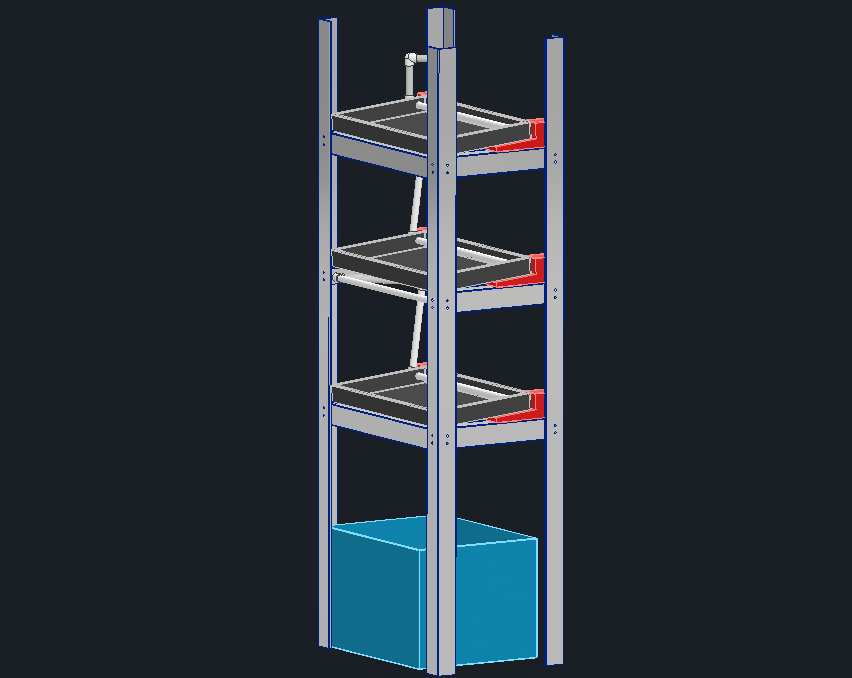
\includegraphics[scale= 0.4]{Figura_17_primera_iteracion_estructura.png}
	\caption{Estructura inicial diseñada utilizando perfiles de aluminio de dos pulgadas.}
	\label{fig:alumin}
\end{figure}

Una vez completado el modelo CAD del sistema, se analizaron los requerimientos de manufactura. Si bien se eliminó la necesidad de realizar soldaduras en aluminio para unir los diferentes perfiles. Esta decisión de diseño implicó agregar una mayor cantidad de agujeros para elementos de fijación mecánicos. Por esta razón, el proceso de fabricación requeriría tanto del corte de los perfiles, utilizando cierra de calar u otras herramientas de corte afines, como el taladrado de agujeros. Adicionalmente, varios de los perfiles, como se observa en la Figura \ref{fig:perfil_h}, contaban con agujeros de diámetros mayores para tuberías, los cuales deberían ser maquinados en una máquina fresadora. Considerando los diferentes procesos de maquinado, se determinó que esta etapa de construcción requeriría de una inversión de tiempo considerable.

\begin{figure}[H]
	\centering
	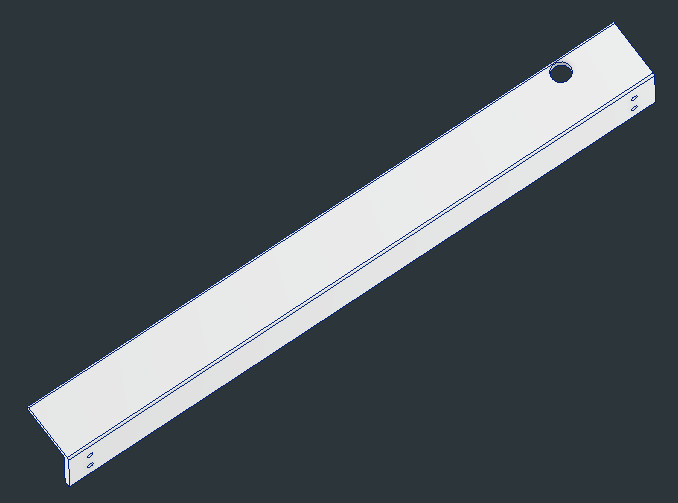
\includegraphics[scale= 0.6]{Perfil_horizontal_aluminio.png}
	\caption{Perfil horizontal con perforación para tubería de distribución.}
	\label{fig:perfil_h}
\end{figure}
\newpage
\subsubsection{Canales de crecimiento}

Como se observa en la Figura \ref{fig:alumin}, en esta iteración se contempló el uso de bandejas de forraje las cuales permitirían el flujo del agua sobre su superficie, logrando así el suministro de nutrientes a las plantas. Adicionalmente, se utilizaron tuberías de PVC de 0.5 pulg, las cuales estarían a cargo de distribuir la solución nutritiva hacia las bandejas de crecimiento y entre cada nivel del sistema. Al utilizar tuberías de distribución para la solución nutritiva, se diseñaron perforaciones que serían necesarias en las bandejas de crecimiento para integrarlas con las tuberías. Adicionalmente, sería necesario implementar una cobertura para las bandejas de crecimiento, que mantuviera oscuro el entorno de las raíces, mientras que brindan una estructura de fijación para las plantas.

\begin{figure}[H]
	\centering
	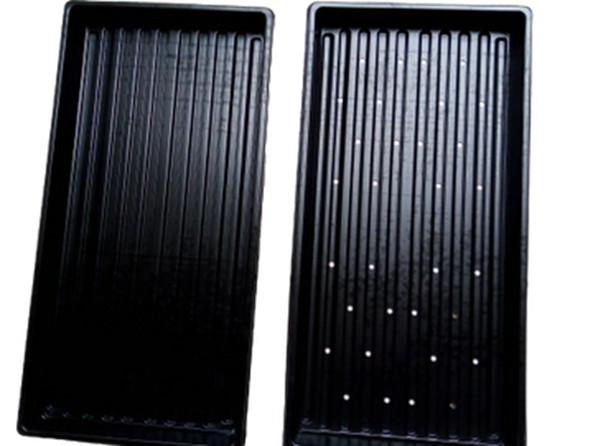
\includegraphics[scale= 0.6]{Bandeja_forraje.png}
	\caption{Bandejas de forraje a utilizarse como canales de crecimiento.}
	\label{fig:bandeja_forraje}
\end{figure}

Una de las ventajas identificadas en las bandejas de forraje fue su versatilidad a la hora de distribuir las plantas. Sin embargo, se observó que las bandejas disponibles en el mercado guatemalteco, ver la Figura \ref{fig:bandeja_forraje}, contaban con canales que limitaban demasiado el flujo de agua, y podrían llevar a puntos secos. Estas áreas sin agua se deben a la irregularidad en el flujo del agua a través de la superficie de las bandejas, lo cual presentaría un riesgo significativo hacia las plantas. Adicionalmente, durante las etapas de diseño se determinó que la cantidad de material necesaria para cubrir las bandejas de crecimiento sería significativa. Estos cobertores para las bandejas requerirían de procesos de impresión por partes, lo cual dificultaría el proceso de construcción. Finalmente, las modificaciones necesarias para asegurar un flujo de agua constante entre las repisas generaría puntos de fuga los cuales podrían llegar a presentar un riesgo para el sistema. Por estas razones, se decidió iniciar una nueva iteración para el diseño del sistema.

\subsection{Segunda iteración, estructura prefabricada}

Si bien la primera iteración permitía una mayor flexibilidad en cuanto al diseño de la estructura, el proceso de fabricación dificultaba cualquier modificación que llegara a ser necesaria. Adicionalmente, al utilizar perfiles de aluminio, esta primera iteración requeriría de una gran cantidad de perfiles de aluminio, los cuales serían difíciles de transportar e instalar. Por esta razón, se inició una segunda iteración buscando utilizar una estructura prefabricada, la cual se pudiera adecuar de manera que fuera funcional en el sistema sin grandes modificaciones.

Luego de unas búsquedas en internet, se encontró una estantería de 1520 mm de altura y 760 mm de ancho. Adicionalmente, contaba con repisas de madera MDF con marcos de metal, las cuales podían ser instaladas a diferentes alturas. Como se observa en la Figura \ref{fig:estanteria_prefab}, se creó un modelo 3D de la estantería, con el cual fue posible observar los beneficios de esta selección en el diseño. Algunas de las ventajas incluyen a las estanterías de madera, las cuales se pueden modificar con facilidad y permiten el uso de tornillos de madera para la fijación de diferentes componentes. Así mismo, los perfiles con ranuras de ojo de cerradura, Figura \ref{fig:Perfil_slotted} se pueden aprovechar para instalar diferentes componentes en el sistema utilizando tornillos y tuercas sin la necesidad de modificar la estructura física. 

\begin{figure}[H]
	\centering
	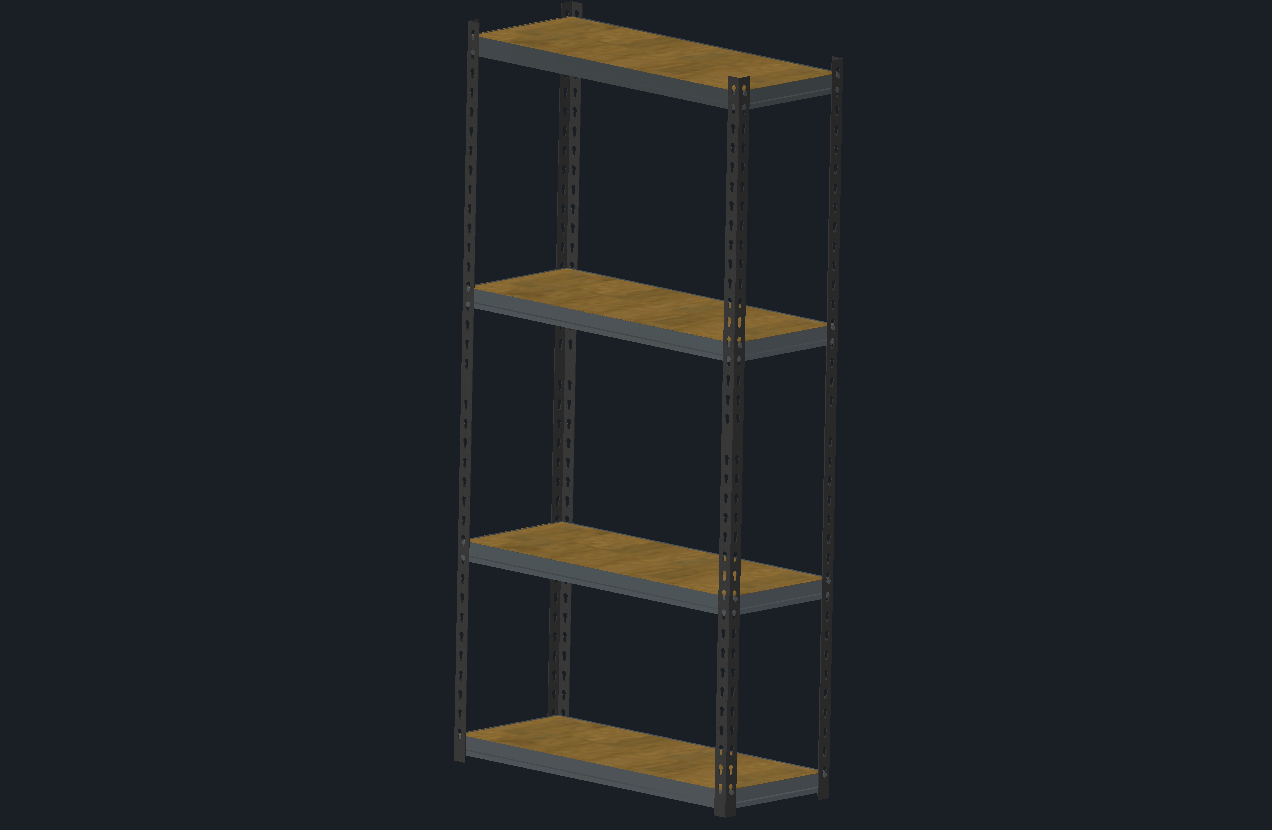
\includegraphics[scale= 0.35]{Estanteria_prefabricada.png}
	\caption{Modelo 3D de la estantería prefabricada.}
	\label{fig:estanteria_prefab}
\end{figure}

\begin{figure}[H]
	\centering
	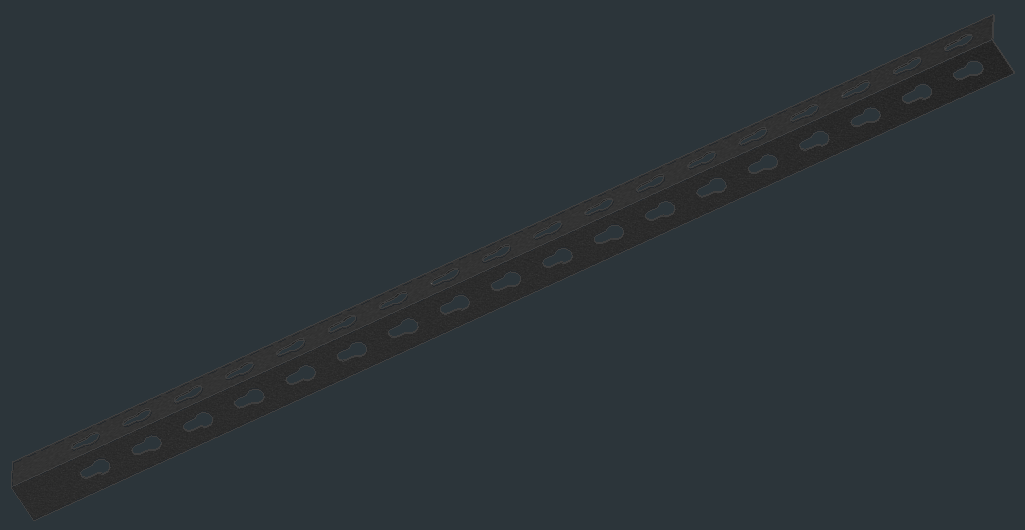
\includegraphics[scale= 0.4]{Perfil_slotted_1.png}
	\caption{Perfil con ranuras de ojo de cerradura.}
	\label{fig:Perfil_slotted}
\end{figure}

\subsubsection{Canales de crecimiento}

Una vez se había definido la estructura de soporte del sistema en la segunda iteración, se continuó con el diseño del sistema de distribución de nutrientes. Con tal de mejorar la canalización del agua y asegurar que las raíces de las plantas recibieran una cantidad adecuada de agua, se seleccionaron tuberías de PVC para los canales de crecimiento de las plantas. Estas tuberías, además de asegurar que el agua se desplazara por una ruta predecible y predeterminada, facilitaban el proceso de construcción. Adicionalmente, estas tuberías de PVC se encontraban con facilidad en el mercado guatemalteco, y no requerían de grandes esfuerzos para su ensamblaje. Por otro lado, el uso de estas tuberías elimina la necesidad de encontrar una forma cubrir los canales de crecimiento, puesto que únicamente es necesario crear agujeros puntuales en la tubería para el crecimiento de las plantas. 

Al tomar en cuenta las consideraciones anteriores, se seleccionaron tuberías de 2.5 pulg, las cuales, junto con uniones de codo a 90° y uniones tipo T, permitirían la elaboración de los canales de crecimiento del sistema. Si bien la mayoría de las modificaciones necesarias para las tuberías consistirían en cortes, agregaron perforaciones de 2 pulg de diámetro las cuales permitirían introducir las canastas de crecimiento en las tuberías. Finalmente, se definió una orientación longitudinal para los canales de crecimiento, la cual permitiría instalar dos tiras de luces de crecimientocon una longitud aproximada de 500 mm en cada nivel. 

\begin{figure}[H]
	\centering
	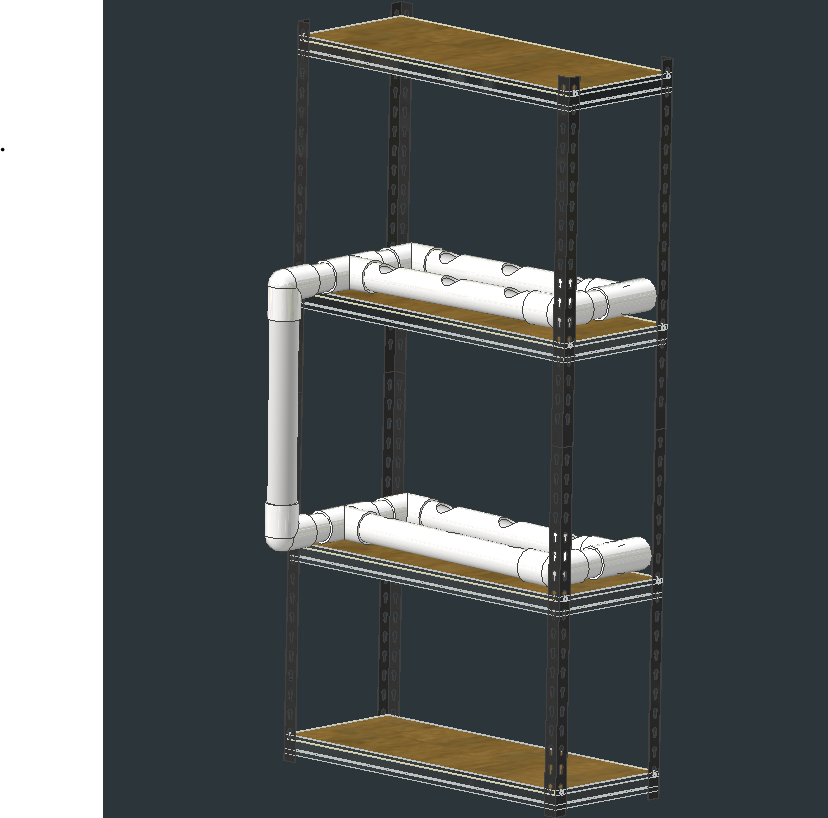
\includegraphics[scale= 0.4]{Canales_crecimiento_estructura.png}
	\caption{Estructura con canales de crecimiento.}
	\label{fig:canales_crecimiento}
\end{figure}

Como se observa en la figura anterior, los canales de distribución de solución nutritiva y de crecimiento, se diseñaron completamente utilizando tuberías y accesorios de PVC. Esta decisión de diseño simplificó considerablemente su ensamblaje mientras que aseguraba un flujo adecuado para las plantas. Si bien las tuberías serían capaces de transportar el agua sin dificultad, aún sería necesaria una inclinación para asegurar el flujo constante de agua. Domando en cuenta la curvatura de las tuberías, se diseñaron dos soportes los cuales permitirían crear tanto una inclinación longitudinal como transversal. Estas inclinaciones serían necesarias para promover el flujo del agua desde el nivel superior hasta el inferior, y a través de las tuberías de crecimiento. Como se observa en la Figura \ref{fig:soporte_tub}, los soportes consistirían de piezas rectangulares con una sección semicircular inclinada a un ángulo de 0.8°, lo cual brindaría la pendiente necesaria para el flujo de agua requerido por el sistema. Estos soportes serían impresos en 3D para facilitar su manufactura, y se utilizarían tornillos para fijarlos a las superficies de las repisas. Cabe mencionar que se crearon dos soportes idénticos de alturas diferentes con tal de obtener una inclinación transversal entre las tuberías y asegurar así el flujo entre niveles.

\begin{figure}[H]
	\centering
	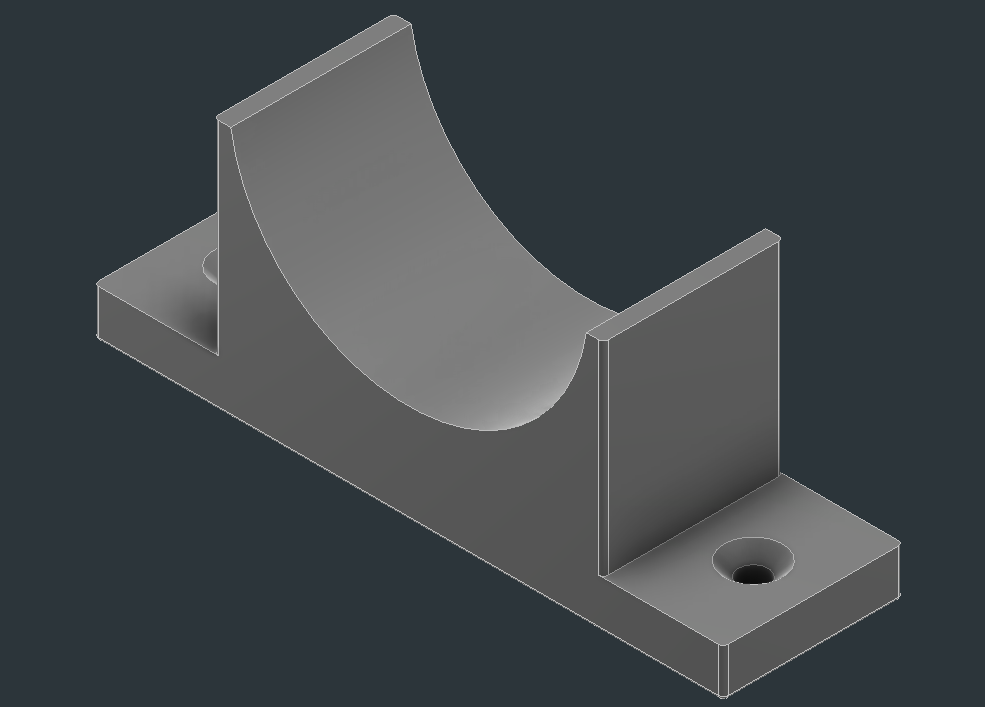
\includegraphics[scale= 0.4]{Soporte_tuberias.png}
	\caption{Soporte con inclinación de 0.8° para tuberías de crecimiento.}
	\label{fig:soporte_tub}
\end{figure}

\subsection{Comparación de las iteraciones de diseño de la estructura}

Si bien la segunda iteración del diseño presentó grande mejoras en cuanto a la facilidad de ensamblaje y construcción, se realizó una comparación entre ambas iteraciones para determinar cuál sería utilizada en el sistema final. A continuación, se encuentra un cuadro comparativo en donde se evaluaron ambas iteraciones respecto a los requerimientos establecidos en la sección 7.1.1. del presente capítulo.

\begin{table}[H]
	\centering
	\begin{tabular}{|c|c|c|} \hline
		~ & \textbf{Primera iteración} & \textbf{Segunda iteración}\\ \hline
		\textbf{Altura max.} & 1750 mm & 1520 mm  \\ \hline
		\textbf{Ancho de repisas} & 586.7 mm & 760 mm \\ \hline
		\textbf{Adaptabilidad} & Pre construcción & Pre y post construcción \\ \hline
		\textbf{Rigidez estructural} & Media & Alta \\ \hline
		\textbf{Resistencia a la corrosión} & Alta & Media \\ \hline
		\textbf{Repisas de madera} & Sin repisas de madera & Repisas de MDF \\ \hline
		\textbf{Facilidad de construcción} & Manufactura compleja & Ensamblaje rápido \\ \hline
	\end{tabular}
	\caption{Análisis comparativo entre primera y segunda iteración de la estructura.}
	\label{cuadro:compar_iter}
\end{table}

Luego de analizar las características del diseño desarrollado para ambas iteraciones como se observa en el Cuadro \ref{cuadro:compar_iter}, se determinó que la segunda iteración sería la más factible para su desarrollo. Esto debido a que cumplió de mejor manera con los requisitos de facilidad de construcción, adaptabilidad \footnote{Esta se ponderó en función de la facilidad de realizar modificaciones una vez se haya instalado el sistema.} y rigidez estructural \footnote{Se determinó que la rigidez estructural de la primera iteración sería menor debido a una mayor altura y menor ancho de repisas, lo cual haría de la estructura menos estable}. Una vez se determinó estructura a utilizar, se iniciaron los procesos de diseño secundarios.

\subsection{Diseño de componentes auxiliares}

Luego del proceso de diseño de la estructura principal, se inició el diseño de los componentes que permitirían integrar la estructura principal con los sensores y actuadores requeridos. Con tal de facilitar el proceso de manufactura, se definieron las siguientes restricciones y consideraciones. Estas deberían ser cumplidas con todos los diseños realizados, asegurando un ensamblaje sencillo.

\begin{itemize}
	\item Simplicidad para impresión 3D: Para modelos pequeños, que su diseño cuente con chaflanes, redondeados y ángulos adecuados con tal de facilitar su manufactura utilizando impresoras 3D con materiales como PLA, ABS o PETG.
	\item Factibilidad de manufactura utilizando corte láser: En caso de que el modelo sea demasiado grande, que este pueda ser fabricado utilizando corte láser con materiales como MDF o acrílico.
	\item Facilidad de ensamble: Que los modelos se puedan ensamblar fácilmente utilizando tornillos u otros medios mecánicos.
\end{itemize}

Utilizando las consideraciones anteriores, se diseñaron dos componentes secundarios. En la Figura \ref{fig:soporte_dht} se observa el primer componente, utilizado para fijar los sensores de temperatura y humedad DHT11 a las repisas de crecimiento. Estos sujetadores para los sensores de DHT11 deberían permitir que se instalaran a una distancia cercana a la altura de las plantas. Esto para asegurar que los parámetros recolectados fueran representativos del entorno alrededor de las hojas y tallos en cada repisa. Para esto se definió el uso de una varilla de madera de 0.5 pulg de diámetro, la cual sería cortada a una longitud aproximada de 160 mm. Los sensores se acoplaron a un anillo, el cual sería fijado a las varillas mediante un tornillo para madera.

\begin{figure}[H]
	\centering
	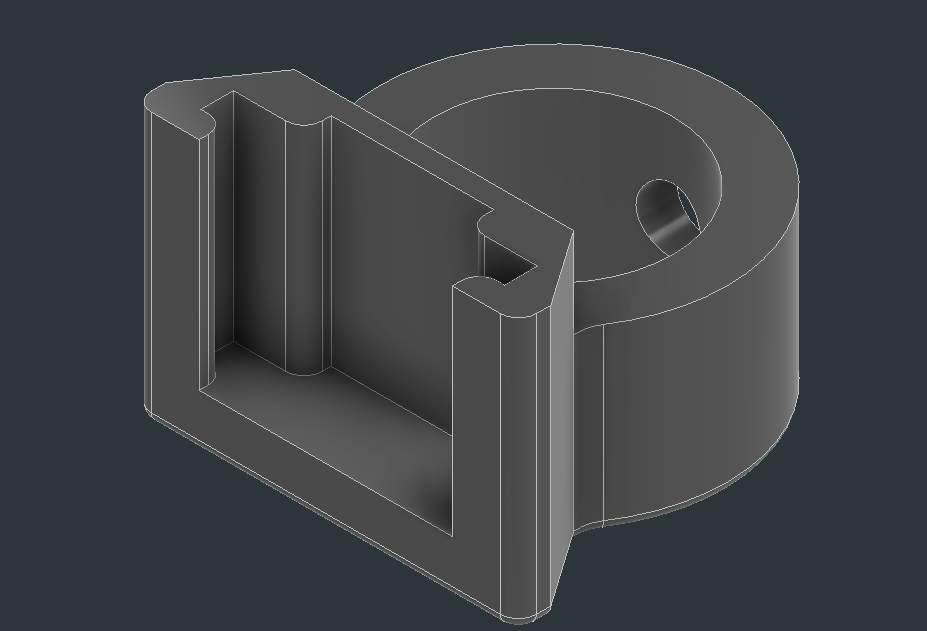
\includegraphics[scale= 0.4]{Soporte_dht11.png}
	\caption{Soporte para sensores DHT11 en varillas de 0.5 pulg.}
	\label{fig:soporte_dht}
\end{figure}

En el caso del segundo componente, este se diseñó para fijar los ventiladores a la estructura de metal. Se diseñaron considerando los agujeros disponibles en cada ventilador para su instalación. Adicionalmente, se diseñó un agujero central que permitiría el uso de tornillos para fijar mecánicamente el soporte a los postes de metal, aprovechando las ranuras de ojo de cerradura. Como se observa en la Figura \ref{fig:soporte_vent}, este componente presenta una baja complejidad, facilitando el proceso de manufactura e instalación.

\begin{figure}[H]
	\centering
	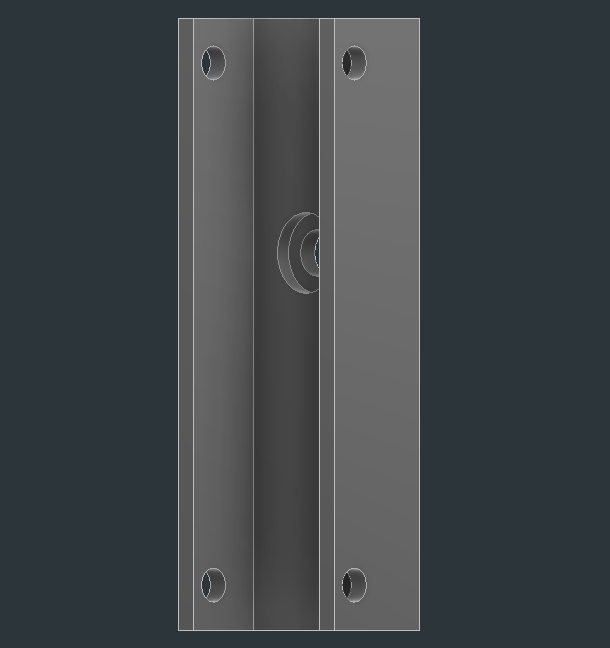
\includegraphics[scale= 0.4]{Soporte_ventilador.png}
	\caption{Soporte para ventiladores con tornillos de 0.25 pulg.}
	\label{fig:soporte_vent}
\end{figure}

\subsection{Modelado CAD de la estructura}

Una vez finalizados los diferentes modelos a instalar en el diseño de la segunda iteración, se integraron todos los componentes para tener un modelo completo del sistema. Como se observa en la Figura \ref{fig:estanteria_v2}, este modelo cuenta con las tuberías de distribución, canales de crecimiento, tanque de almacenamiento de agua. Además, cuenta con las varillas para la sujeción de los sensores y demás componentes auxiliares.

\begin{figure}[H]
	\centering
	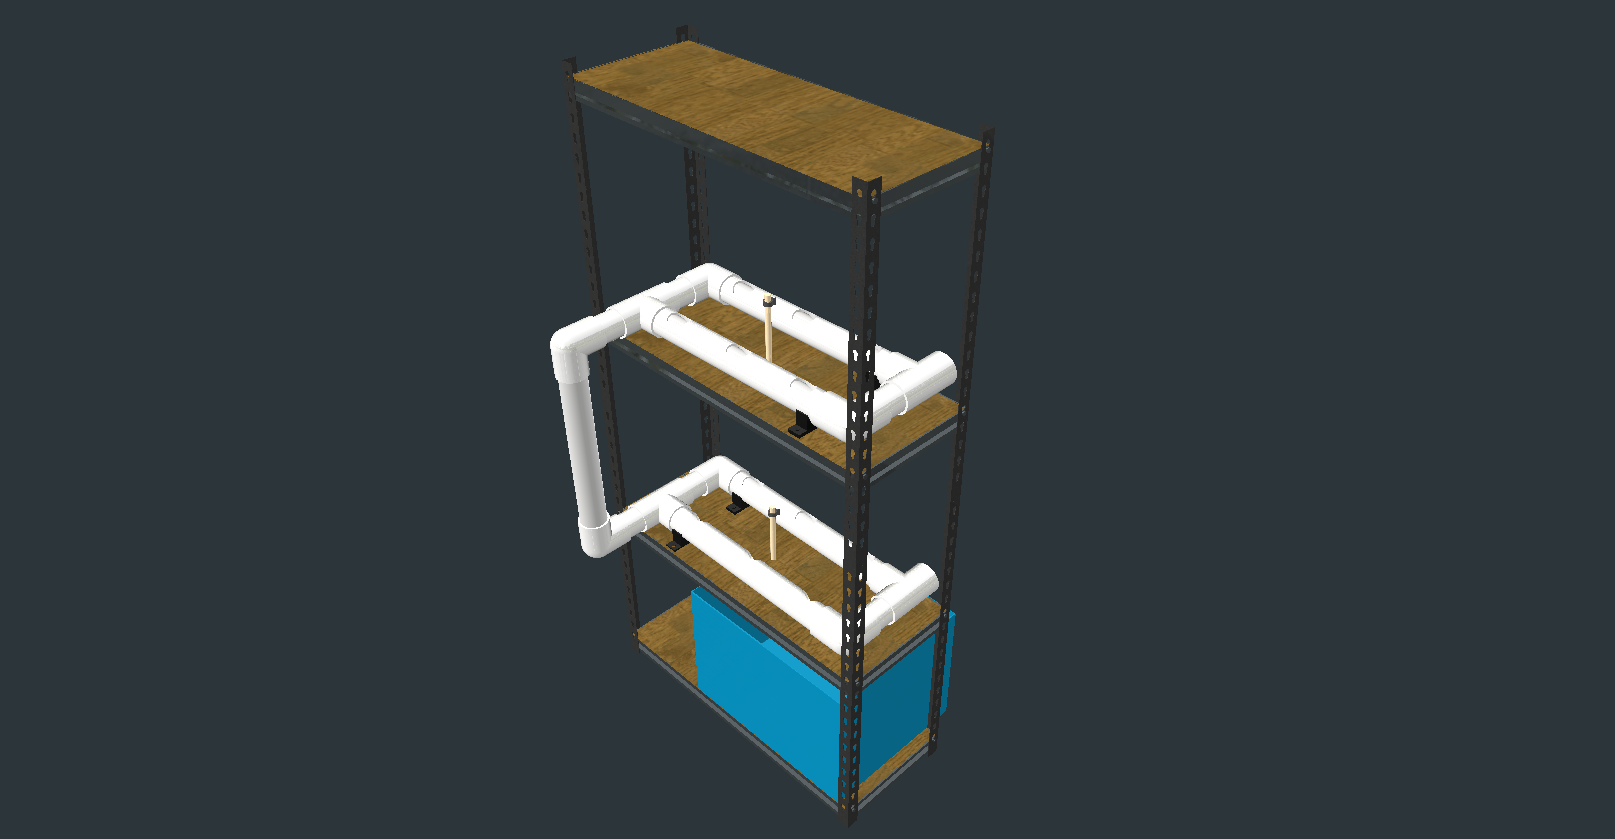
\includegraphics[scale= 0.4]{TH_ensamble_prototipo_v2.png}
	\caption{Ensamblaje del modelo CAD de la estructura principal del sistema.}
	\label{fig:estanteria_v2}
\end{figure}

Con este modelo establecido, fue posible continuar con el proceso de construcción, el cual se discutirá en la sección 7.3. del presente capítulo.

\section{Diseño de circuitos}

El sistema de control se basó en el microcontrolador ESP-WROOM32 y la placa de desarrollo de \textit{Hiletgo} ESP-32S. Esta placa se utilizó para obtener información de los diferentes sensores y activar los actuadores conectados al sistema. Debido al uso de un microcontrolador con una placa de desarrollo, la mayor parte de los circuitos del sistema se categorizaron como conexiones de componentes digitales. Si bien esto redujo la complejidad del proceso en el diseño de los circuitos, se encontraron varios retos relacionados a niveles de voltaje y disponibilidad de conexiones en la placa de desarrollo. A continuación, se detallan las diferentes etapas consideradas en el diseño del sistema electrónico.

\subsection{Características de alimentación de potencia}

Desde el controlador hasta los sensores, luces y actuadores requieren de una alimentación regulada de voltaje CC (corriente continua). Como se discutió en el capítulo 6, la mayoría de los componentes utilizados cuentan con un rango de voltaje de operación entre los 3 y 5.5 voltios CC. Por otro lado, los ventiladores a utilizar en el sistema consistirían de ventiladores de corriente alterna, por lo que sería necesario acceso a una línea de 120 voltios CA (corriente alterna). Por estas razones, la fuente seleccionada debería ser capaz de entregar un voltaje de 5 voltios CC y ser capaz de funcionar con una entrada de 120 voltios CA. Adicionalmente, en el capítulo 6 se detallaron las características de consumo de corriente de los sensores a utilizar, con las cuales se calculó un consumo máximo de corriente de 5 amperios, según se observa en el Cuardo \ref{cuadro:corriente_sensores}.

\begin{table}[H]
	\centering
	\begin{tabular}{|c|c|c|} \hline
		\textbf{Componente} & \multicolumn{2}{c|}{\textbf{Corriente máxima}} \\ \hline
		2 sensores DHT11 & 10 & $mA$ \\ \hline
		3 sensores DS18B20 & 12 & $mA$ \\ \hline
		Sensor PH SEN0161 & 600 & $mA$ \\ \hline
		Sensor DFR0300 & 600 & $mA$ \\ \hline
		Sensor SEN0237 & 600 & $mA$ \\ \hline
		Relé Shori S3H-5-1C-S & 72 & $mA$ \\ \hline
		RTC DS3231 & 575 & $\mu A$ \\ \hline
		ESP-WROOM-32 & 1.5 & $A$ \\ \hline
		Total: & 3.4 & $A$ \\ \hline
	\end{tabular}
	\caption{Corriente máxima requerida por los componentes del circuito.}
	\label{cuadro:corriente_sensores}
\end{table}

Al considerar el consumo de corriente total de los componentes principales, así como las demás características mencionadas, se seleccionó una fuente de alimentación conmutada de 5 voltios a 5 amperios. Se optó por esta fuente puesto que se alimentaba utilizando 120 voltios CA, dejando terminales de conexión disponibles para conexiones de 120 VCA y los 5 VCC, requeridos. Adicionalmente, estas fuentes cuentan con una salida de voltaje estable, gracias a su control por variación de ancho de pulso, asegurando un voltaje constante.

\subsubsection{Pruebas físicas de circuitos principales}

Una vez seleccionada la fuente de alimentación, se realizaron una serie de pruebas con los diferentes componentes del sistema. Estas se dividieron en tres etapas, una para pruebas con sensores de temperatura, otra para ventiladores, y una última para luces de crecimiento. Luego de estas pruebas, se inició el proceso de integración de componentes, implementando los ajustes que se consideraron necesarios.

Durante la primera etapa de pruebas, se conectaron los sensores DHT11 junto con los sensores de temperatura de agua DS18B20. Adicionalmente, se conectó el microcontrolador, el cual contaba con la programación requerida para la lectura de los valores entregados por los sensores de temperatura. En esta etapa de pruebas, se determinó que la corriente y el voltaje eran suficientes para el funcionamiento adecuado de los sensores. Ahora bien, se detectaron ciertos fallos de conexión, los cuales llevaron a caídas de voltaje inesperados. Por otro lado, en la segunda etapa de pruebas, se conectaron los ventiladores utilizando relés transistorizados. Durante estas pruebas, se confirmó el funcionamiento de los relés y ventiladores, los cuales estarían combinando un circuito de 120 voltios CA y 5 voltios CC. Finalmente, en la tercera etapa se conectaron las tiras de leds, las cuales en combinación, llegaron a una longitud de 2 metros. De las pruebas realizadas, la prueba con las tiras de luces led presentó problemas respecto a la demanda de corriente de las tiras. Como se demuestra a continuación, el consumo de las tiras de luces led incrementó considerablemente, por lo que se volvió a evaluar el consumo del sistema \footnote{Luego de investigar la hoja de datos de las luces utilizadas, se encontró que estas contaban con un consumo máximo de 0.036 $mA$ por luz, por lo que una tira de 120 luces, contaría con un consumo total de 4.32 $A$.}.

\begin{table}[H]
	\centering
	\begin{tabular}{|c|c|c|} \hline
		\textbf{Componente} & \multicolumn{2}{c|}{\textbf{Corriente máxima}} \\ \hline
		2 sensores DHT11 & 10 & $mA$ \\ \hline
		3 sensores DS18B20 & 12 & $mA$ \\ \hline
		Sensor PH SEN0161 & 600 & $mA$ \\ \hline
		Sensor DFR0300 & 600 & $mA$ \\ \hline
		Sensor SEN0237 & 600 & $mA$ \\ \hline
		Relé Shori S3H-5-1C-S & 72 & $mA$ \\ \hline
		RTC DS3231 & 575 & $\mu A$ \\ \hline
		ESP-WROOM-32 & 1.5 & $A$ \\ \hline
		Neopixel WS2812B & 4.32 & $A$ \\ \hline
		2 servomotores MG90S & 1.6 & $A$ \\ \hline
		Total: & 9.31 & $A$ \\ \hline
	\end{tabular}
	\caption{Corriente máxima requerida por el sistema completo de voltaje CC.}
	\label{cuadro:corriente_maxima}
\end{table}

Al analizar nuevamente el consumo de corriente, se determinó que sería necesaria una fuente de alimentación conmutada capaz de entregar como mínimo 10A. Si bien durante el funcionamiento del sistema completo, no todos los componentes estarían consumiendo su corriente máxima al mismo tiempo, esta es una posibilidad que no se debe descartar. Con tal de mejorar el factor de seguridad, se consideró el uso de una fuente conmutada de 15 amperios, sin embargo, no se encontraban disponibles en el país al momento de realizar las pruebas.

Gracias a las pruebas realizadas, se observaron ciertos cambios en el comportamiento del microcontrolador en diferentes etapas de funcionamiento del circuito. Se observó que durante ciclos de conexión a una red WiFi, así como durante el uso de las luces de crecimiento, el microcontrolador tendía a perder potencia. Esto a pesar de que el módulo de conversión de voltaje disponible en la placa de desarrollo es considerablemente robusto ante variaciones de voltaje. Debido a esto, se consideró la implementación de un banco de capacitores. Dicha modificación al circuito logró estabilizar el voltaje de alimentación del ESP-32S y presentó mejoras considerables durante los ciclos mencionados.

\subsection{Configuración de conexiones para sensores y actuadores}

Durante la etapa de diseño del circuito, fue necesario incluir componentes analógicos necesarios para la regulación del voltaje y para mantener sus características de funcionamiento. Estos se resumen en resistencias y transistores, los cuales se utilizaron para regular la corriente en pines específicos. 

\subsubsection{Circuito de control de relés}

El microcontrolador ESP-32S, cuenta con salidas lógicas en sus pines digitales de 0 a 3.3 voltios CC, lo cual no sería capaz de controlar los relés de 5 voltios CC utilizados en el sistema. Por esta razón, se utilizó un transistor BJT, el cual sería capaz de controlar el flujo de corriente entre su colector y emisor utilizando el voltaje de la señal digital del microcontrolador. Al tomar en cuenta este requerimiento en el diseño, se calculó la corriente de saturación del transistor al ser alimentado con 3.3 voltios CC.

\begin{table}[H]
	\centering
	\begin{tabular}{|c|c|c|} \hline
		\multicolumn{3}{|c|}{\textbf{Características principales}} \\ \hline
		Ganancia DC ($\beta$) & 100 & ~ \\ \hline
		Corriente de saturación & $I_B$=15 & $mA$ \\ \hline
		Voltaje de saturación $V_{BE}$ & 1.2 & $V$ \\ \hline
		Corriente requerida $I_C$ & 72 & $mA$ \\ \hline
	\end{tabular}
	\caption{Características de los transistores NPN 2N222A y del circuito.}
	\label{cuadro:2n222a_caracter}
\end{table}

Con tal de calcular la resistencia de base necesaria para controlar los relés, se emplearon las siguientes ecuaciones:

\begin{equation}
	I_B = \frac{I_C}{\beta}
	\label{eq:I_B_colector}
\end{equation}

\begin{equation}
	I_B = \frac{V_B-V_{BE}}{R_B}
	\label{eq:I_B_resistor}
\end{equation}

De la ecuación \ref{eq:I_B_colector} se obtuvo una corriente de base $I_B = 72$ $\mu A$. Ahora bien, esta corriente no sería suficiente para saturar el transistor, como se observa en el Cuadro \ref{cuadro:2n222a_caracter}, la corriente de saturación debe ser de 15 $mA$. Utilizando esta corriente, se calculó el valor de la resistencia a utilizar, considerando que el voltaje de la base en su estado activo sería de $V_{B} = 3.3$ V. De la Ecuación \ref{eq:I_B_resistor} se despejó para la resistencia. Al ingresar los valores requeridos en la ecuación despejada se obtuvo $R_B = \frac{3.3V-1.2V}{0.015mA}$, resultando en un valor de $R_B = 140$ $\Omega$.

Con tal de utilizar un valor de resistencia comercialmente disponible, se propuso el uso de resistencias de 100 $\Omega$. Se realizó una comprobación aplicando la Ecuación \ref{eq:I_B_resistor}, con la cual se obtuvo una corriente base $I_B = 21$ $mA$. Al tomar en cuenta que para lograr la saturación, se debe cumplir la siguiente relación: $I_C < \beta I_B$, se determinó que la resistencia seleccionada sería adecuada para activar el relé a utilizar. Del análisis anterior, se derivó el diagrama de la Figura \ref{fig:diag_rele}.

\begin{figure}[H]
	\centering
	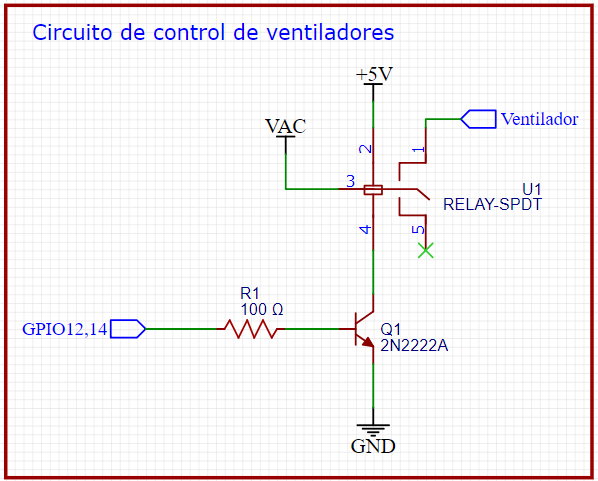
\includegraphics[scale= 0.4]{Circuito_ventiladores.png}
	\caption{Circuito con resistencia calculada para control de ventiladores con relés de 5 VCC.}
	\label{fig:diag_rele}
\end{figure}

Como se observa en el diagrama, los circuitos de control del ventilador inferior y superior se conectaron a los pines de uso múltiple 12 y 14 respectivamente. 

\subsubsection{Sensores de temperatura}

En el caso de los sensores de temperatura DHT11 y DS18B20, estos se conectaron según las recomendaciones del fabricante. Para los sensores DHT11 se utilizaron resistencias de $10k$ $\Omega$ conectadas entre 5 VCC y el pin de datos. Para estos sensores, se utilizaron los pines de uso general 4 y 13 del microcontrolador. Por otro lado, en los sensores DS18B20 se utilizó una única resistencia de $4.7k$ $\Omega$ conectada entre 5 VCC y el bus de datos. Debido al uso del protocolo One-wire, se utilizó un bus de datos conectado al pin de uso general número 15.

\subsubsection{Módulo RTC y luces de crecimiento}

El módulo de reloj de tiempo real DS3231 y las luces de crecimiento presentaron la conexión más sencilla. En estos componentes, no se utilizaron resistencias adicionales. En el caso del reloj de tiempo real, este se conectó a los pines de uso general 22 y 21, los cuales corresponden a la señal SCL y SDA respectivamente. Finalmente, las luces de crecimiento se conectaron al pin número 27.

\subsection{Desarrollo de placa PCB}			% [==========MISSING==========]

\section{Construcción del sistema}

Una vez completado el proceso de diseño general, se inició la construcción física del sistema. Como primer paso, se ensambló la estantería de metal, la cual sería utilizada como estructura principal para el sistema. Este proceso se logró con la ayuda de un mazo de goma y un metro, con los cuales se fijaron las repisas de la estantería a las alturas definidas en la etapa de diseño. Adicionalmente, se modificó una de las repisas con tal de asegurar un flujo adecuado de aire dentro del sistema. Estas modificaciones se realizaron utilizando un router manual con una fresa de 0.5 pulg con el cual se crearon ranuras longitudinales en la repisa de MDF. Una vez ensamblada la estructura principal, se inició con el ensamblaje de las tuberías de distribución y crecimiento.

El ensamblaje de las tuberías de crecimiento se inició con una tubería de 3 metros de largo, con un diámetro de 2 pulg. Esta tubería se cortó en las diferentes secciones requeridas para la construcción de los canales de crecimiento y tuberías de distribución. Luego, se utilizó una broca de copa de 1.5 pulg para realizar perforaciones en los canales de crecimiento espaciados a 17.54 mm. Estos agujeros serían utilizados para contener las plantas durante el período de crecimiento. Una vez se habían recortado todas las secciones de PVC, se utilizó sellador de silicona con una pureza del 100\% para unir las piezas con los codos y uniones tipo T. Se utilizó esta silicona para asegurar que no se encontraran fugas en los canales de distribución o crecimiento. Adicionalmente, la pureza aseguró que no se encontraran contaminantes los cuales podrían interferir con las pruebas a realizar. Finalmente, se conectó una manguera flexible de 0.5 pulg de diámetro interno al inicio de los canales de distribución, la cual permitiría suministrar el agua utilizando una bomba sumergible.

\subsection{Integración de sistemas}

Una vez se contaba con la estructura principal ensamblada, se inició la instalación de los diferentes componentes eléctricos y electrónicos en el sistema. Se instaló una caja plástica de 32 litros, la cual funcionaría como sistema de almacenamiento de agua. Una vez instalado dicho contenedor, se continuó con la instalación y conexión de sensores, actuadores, y la bomba sumergible.

\subsubsection{Conexión de sensores}

Tanto los sensores de temperatura ambiental como del agua requirieron de pequeñas modificaciones para su instalación. En el caso de los sensores DHT11, se crearon cables de conexión utilizando alambres de un cable UTP. Estos se unieron a terminales de pines axiales los cuales se utilizaron para conectar los cables a cada sensor y a la placa de desarrollo. Por otro lado, los sensores DS18B20 ya contaban con cables suficientemente largos, con la excepción de uno, por lo que se soldaron pines axiales directamente a los cables de los sensores. En el caso del sensor de temperatura de agua que se encontraba más alejado de la placa de desarrollo, se utilizó cable UTP para crear las extensiones requeridas. Finalmente, el sensor de pH SEN0161 cuenta con cables con terminales de pines axiales, por lo que la conexión no requirió de modificaciones a los cables existentes.

Los sensores DHT11 se instalaron utilizando las piezas impresas en 3D mencionadas al inicio del capítulo. Se utilizaron las varillas de 0.5 pulg para fijar los anillos de los sensores, y estas se insertaron directamente en la madera de las repisas. En el caso de las sondas de temperatura de agua, se introdujeron mediante los agujeros diseñados para fijar las plantas. Estas se ubicaron en cada una de las repisas de crecimiento, asegurando tomar mediciones en el punto de inicio del flujo de agua. La tercera sonda de temperatura de agua se instaló directamente en el depósito central de agua. 

\subsubsection{Instalación de bomba de circulación de agua}

La bomba de circulación de agua utilizada se acopló a la manguera flexible utilizando una boquilla de 0.5 pulg de diámetro, la cual se insertó a presión dentro de la manguera. Se aseguró que la distancia de la bomba hacia el punto de salida de la manguera se encontrara dentro de un rango de 3.5 pies, con tal de no forzar la bomba y asegurar un flujo adecuado de agua. Finalmente, la bomba se sumergió en el agua, y se fijó utilizando ventosas al fondo del depósito plástico. Se aseguró que la conexión del cable se encontrara lo más alejada de la fuente de agua posible, para evitar fallos por corto circuito.

\subsubsection{Instalación de actuadores}

Durante las primeras fases de construcción, se instalaron los ventiladores utilizando sus bases impresas, las cuales se fijaron mediante tornillos y tuercas a los perfiles de metal de la estructura principal. Al igual que los sensores, se soldaron extensiones de cable UTP a los ventiladores, permitiendo que los cables llegaran a sus puntos de conexión en la placa de desarrollo. Adicionalmente, se cubrieron todos los empalmes utilizando cinta de aislar, con tal de evitar fallos por corto circuito. Por otro lado, las luces de crecimiento se instalaron utilizando repisas adicionales, suspendidas a una distancia de aproximadamente 150 mm de las tuberías de crecimiento. Se utilizó cable UTP para unir las diferentes secciones de tiras LED, y se colocaron conectores axiales en cada una de las secciones, asegurando así una fácil conexión entre la placa de desarrollo y las luces de crecimiento.

\begin{figure}[H]
	\centering
	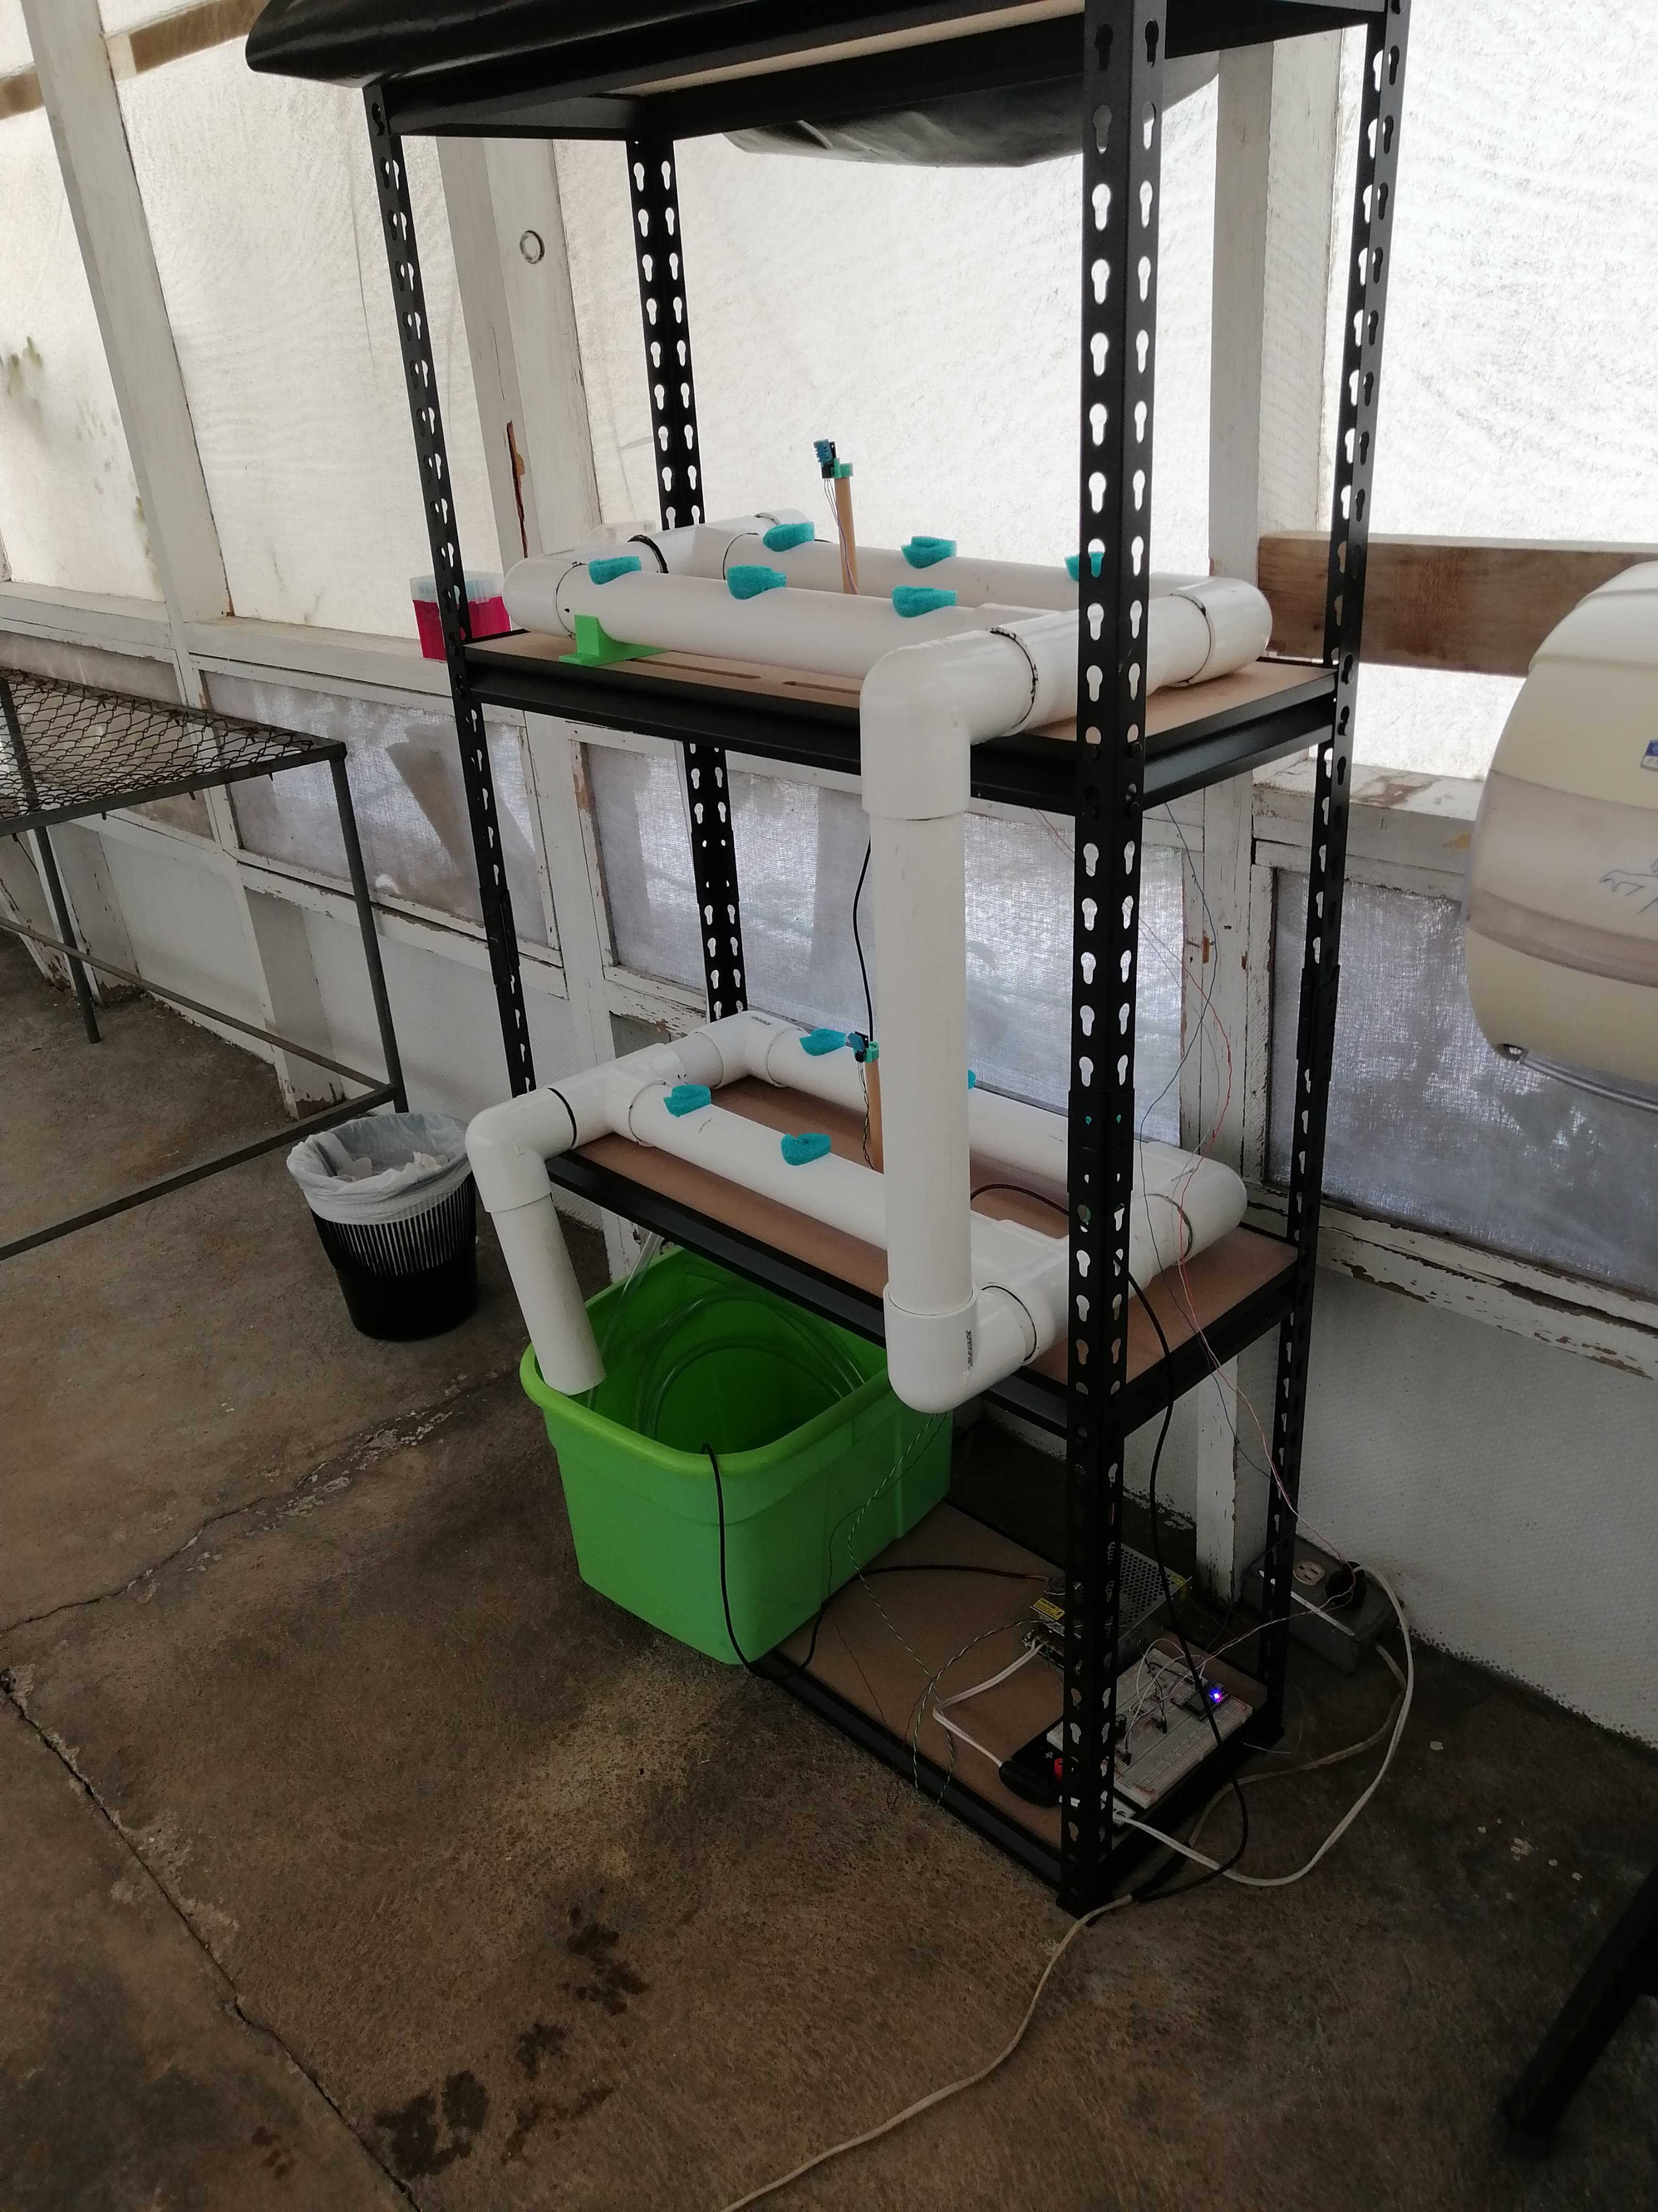
\includegraphics[scale= 0.05]{Estructura_principal.jpg}
	\caption{Estructura instalada en vivero con los diferentes componentes instalados y conectados.}
	\label{fig:estructura_final}
\end{figure}

%-----------------------------------------------------------------------------------------------------------

\chapter{Programación del \textit{firmware} del sistema}

\section{Definición de protocolo de comunicación inalámbrica}

Una de las ventajas de los sistemas hidropónicos se centra en sus bajos requisitos de mano de obra y atención constante. Esta ventaja se puede capitalizar significativamente al incluir un protocolo que permita enviar los datos a un servidor para ser consultados por un operador de manera remota. En el Siglo XXI, el crecimiento de tecnologías inalámbricas han facilitado esta tarea mediante el Internet de las cosas (IoT, por sus siglas en inglés). Si bien el internet de las cosas es un concepto sumamente valioso, este no se puede aprovechar sin contar con un protocolo de comunicación de datos que habilite su acceso.

\subsection{Conexión inalámbrica mediante WiFi}

El crecimiento en popularidad del internet de las cosas se atribuye principalmente a los avances realizados en cuanto a la familia de protocolos de comunicación con fidelidad inalámbrica, más conocida como WiFi. \cite{biber} Esta familia de protocolos ofrece una gran flexibilidad en cuanto a la estructura de paquetes para el envío de datos a través de grandes distancias y de una gran variedad de dispositivos. Esta versatilidad, permite a microcontroladores y plataformas de desarrollo como el ESP-WROOM32 utilizar este protocolo de comunicación para la transferencia de datos de manera inalámbrica.

Se utilizó la librería de \textit{WiFi.h} para la conexión del ESP-WROOM32 a una red local de internet. Una de las prioridades a la hora de diseñar la conexión a internet fue asegurar que el resto del sistema de control mantuviera su funcionamiento en caso de que se perdiera conexión WiFi. Tomando esto en cuenta, se estableció un intento inicial de conexión una vez se enciende el sistema. En caso de que se haya perdido conexión, o esta no se haya establecido exitosamente, se estableció un período de espera de 30 minutos, durante los cuales el sistema no intentaría conectarse al internet. Finalizados los 30 minutos, el sistema iniciaría nuevamente su rutina para establecer dicha conexión. Esta implementación fue esencial, puesto que la rutina para conectar el sistema al internet bloquearía el código durante un período considerable de tiempo. Por esta razón, sería necesario salir de la rutina de conexión luego de cierto tiempo, antes de volver a intentar la conexión.

\subsubsection{Protocolo HTTP}

Una vez establecida la conexión WiFi, se habilitó la comunicación con el servidro de Dweet.io mediante el protocolo HTTP. Puesto que la comunicación HTTP consiste de una solicitud enviada a un servidor, esta no requiere establecer una conexión como tal. Por esta razón, se programó una función a cargo de envíos de datos al servidor, iniciando la solicitud en el momento deseado, y finalizando una vez se recibió una respuesta adecuada del servidor. Debido a que una interrupción en el envío de datos podría resultar en un error, se estableció una cantidad de intentos máxima, para asegurar que los datos fuesen enviados, o que se regresara al ciclo principal en caso de no lograr la comunicación. Al igual que la función para la conexión a la red WiFi, la comunicación HTTP bloqueaba el código durante un tiempo significativo, por lo que estas medidas de seguridad se consideraron justificables.

Durante cada conexión al servidor, se enviaron dos paquetes de información, uno a la dirección \textit{hydro\_test} y otro a la dirección \textit{hydro\_LOG}. El primero de estos paquetes consistió de datos de los sensores, estados de los actuadores, e información de la fecha y hora del reloj de tiempo real del sistema. Esta información sería procesada por la aplicación con tal de monitorear los parámetros dentro del sistema de crecimiento. El segundo de los paquetes consistió de información acerca del estado de la conexión, detallando el nombre de la red a la que se encuentra conectado el sistema, así como la intensidad de la señal, la fecha y hora, y un contador de la cantidad de veces que falló el envío de datos al servidor antes del envío actual. Es importante mencionar que la información en ambos paquetes se configuró utilizando el formato JSON, el cual establece un objeto compuesto por un conjunto de propiedades, a las cuales se les asigna un valor según sea necesario. En este caso, se utilizó el formato JSON para establecer propiedades de temperatura, humedad, y otros parámetros los cuales se unieron con los valores recolectados por los sensores.

\section{Configuración de sensores y accionamiento de actuadores}

El proceso de configuración de los sensores de temperatura y humedad, así como las sondas de temperatura del agua, se completó sin mayor dificultad. Esto pues, la simplicidad en el funcionamiento de estos sensores eliminó los requerimientos de calibración. Los valores obtenidos de estos sensores se compararon con límites preestablecido, con tal de definir una secuencia de control sencilla para los ventiladores. Esto se implementó con tal de asegurar que tanto la temperatura como la humedad ambiental se mantuvieran en un rango adecuado para el crecimiento de las plantas. Por otro lado, los datos recolectados de las sondas de temperatura se almacenaron para ser enviadas al servidor de Dweet.io para su monitoreo.

En el caso de los actuadores, se establecieron funciones de control para los ventiladores y las luces de crecimiento respectivamente. En el caso de la función para la activación de los ventiladores, esta se enfocó en activar los pines transistorizados para cada ventilador, y cambiar el estado de banderas específicas con tal de comunicar el estado de los ventiladores al operador. Ahora bien, el control de las luces de crecimiento presentó una mayor cantidad de retos. Si bien la función diseñada para encender y apagar las luces de crecimiento no presentó grandes obstáculos, permitiendo cambiar el color de cada luz de manera individual y encender las luces a intervalos establecidos, se dificultó el registro del tiempo. Debido a los requerimientos de luz de las plantas, las luces de crecimiento deberían permanecer encendidas durante un período determinado. Ahora bien, se debería mantener un punto de referencia, con el cual se podría establecer cuánto tiempo han estado encendidas las luces, y cuanto tiempo más deberían estar apagadas, aún cuando el sistema de control perdiera alimentación. Por esta razón, se introdujo el módulo RTC, el cual aseguraría que las luces se encendieran siempre a la hora configurada, y se apagaran a la hora deseada. Durante la configuración del módulo RTC, se incluyó una rutina para sincronizar el tiempo del reloj interno con el tiempo del servidor de Dweet.io en caso de que el módulo perdiera poder. Estas medidas aseguraron que el tiempo del sistema se mantuviera de acuerdo con el tiempo real de la ubicación del sistema.

%------------------------------------------------------------------------------------------------------------

\chapter{Desarrollo de aplicación móvil}

\section{Requisitos de funcionalidad}

La aplicación móvil presenta una oportunidad de desarrollar una interfaz demostrativa, que sea capaz de brindar información al usuario de manera legible. Por esta razón, se establecieron diferentes requisitos de funcionalidad. Uno de estos, consistió en la conexión de la aplicación a internet para establecer una comunicación con el servidor de Dweet.io y obtener los datos del sistema. Otro de los requisitos de funcionalidad se centró en contar con una interfaz fácil de leer, que desplegara los datos recolectados por los sensores al usuario de una manera sencilla. De la mano con este requisito, se estableció que el usuario no fuese capaz de ingresar datos en las casillas que desplegaran los datos de los sensores. Finalmente, se buscó que la interfaz contara con un botón que permitiera al usuario refrescar los datos con tal de asegurar que la lectura más actualizada de los sensores se estuviese desplegando en la interfaz. 

\subsection{Diseño de interfaz gráfica}

El diseño de la interfaz gráfica se llevó a cabo utilizando el lenguaje de marcado extensible XML. Dentro del entorno de programación del estudio de \textit{Android}, se definieron dos pantallas. Una de estas presentaría el logo de la aplicación, así como el nombre, mientras que la segunda contaría con la información de los sensores del sistema. Se desarrolló el logo de la aplicación utilizando la herramienta gratuita de \textit{Canva}, y se utilizaron las herramientas de \textit{Android} para importar las imágenes utilizadas en la aplicación. Una vez se definieron las pantallas, sus estructuras y sus componentes, se continuó con la programación del funcionamiento de la aplicación.

\begin{figure}[H]
	\centering
	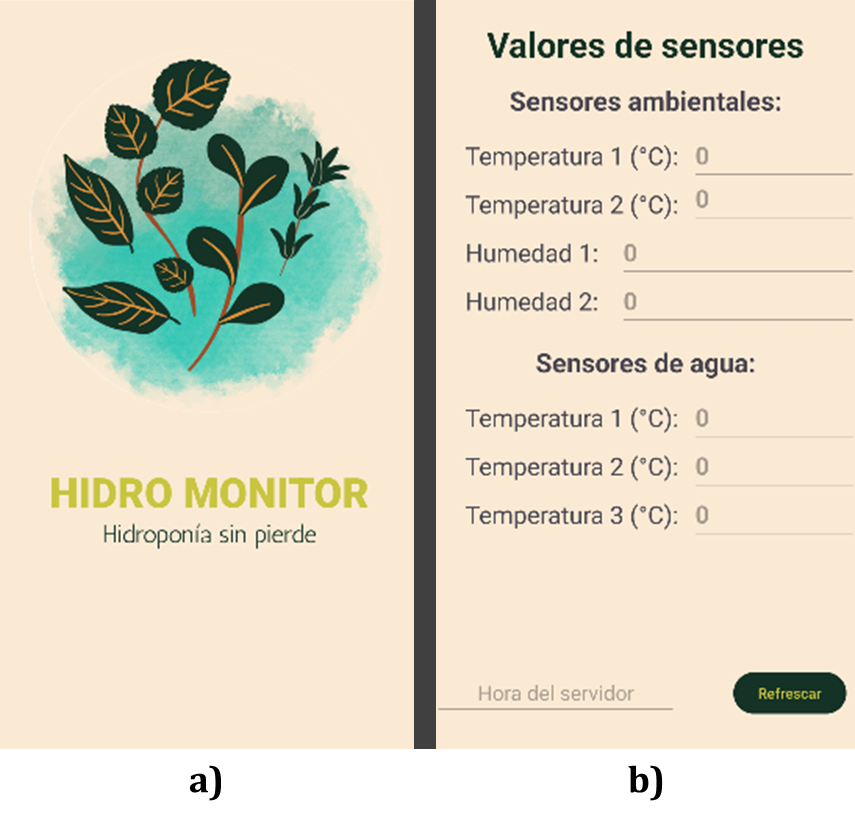
\includegraphics[scale= 0.5]{Interfaz_grafica.png}
	\caption{a) Pantalla de inicio de la aplicación. b) Interfaz gráfica principal.}
	\label{fig:interfaz_graf}
\end{figure}

\subsection{Lectura de datos de servidor HTTP}

Se utilizó el protocolo HTTP para obtener los datos del servidor Dweet.io bajo la dirección de \textit{hydro\_test}. Dentro de la función de lectura de datos del servidor, se obtuvieron los valores de las categorías del objeto JSON, y se asignaron a variables las cuales serán utilizadas para actualizar las casillas respectivas en la interfaz. Adicionalmente, se estableció un ciclo de lectura continuo, el cual realizaría una solicitud de información al servidor cada 5 minutos, e iniciaría un segundo después de acceder a la interfaz. Finalmente, se incluyó una función que ejecutaría una solicitud al servidor en el caso de que se presionara el botón para refrescar los datos.

\subsection{Notificaciones}					% [==========MISSING==========]

%-------------------------------------------------------------------------------------------------------------

\chapter{Evaluación del crecimiento del cilantro}

\section{Cultivo del cilantro en sustrato nutritivo}

Con tal de evaluar el crecimiento del cilantro, se inició un cultivo utilizando un sustrato activo. Este cultivo funcionaría como punto de comparación, permitiendo identificar cambios en el crecimiento del cilantro dentro del sistema. Con tal de lograr el crecimiento adecuado de las plantas de cilantro, se estableció un sustrato que fuese capaz de cumplir con las siguientes características: alta retención de humedad, baja densidad permitiendo oxigenación y un alto contenido nutritivo. Con estas características en mente, se realizó una mezcla de vermiculita, \textit{peat-moss}, tierra abonada y compost orgánico. Esta mezcla permitió contar con una buena retención de agua gracias a la vermiculita, un nivel bajo de densidad debido al \textit{peat-moss}, y una alta cantidad de nutrientes. Una vez se preparó el sustrato de crecimiento, se repartió en diferentes contenedores, los cuales permitirían el desarrollo de las plantas asegurando una distancia de 180 mm entre planta. 

\subsection{Período de germinación del cilantro}

Con tal de establecer una línea base de crecimiento, se inició un grupo de plantas de cilantro desde la semilla. Para esto, se emplearon dos metodologías de germinación. En la primera, como se observa en la Figura \ref{fig:ziplock} se utilizó una bolsa resellable, en la cual se introdujo una toalla de papel húmeda con semillas de cilantro. Esta bolsa se almacenó en un ambiente oscuro y a una temperatura constante cercana a los 25 °C. Como segundo método, se utilizó un sustrato inerte, el cual consistió en una mezcla de \textit{peat-moss}, vermiculita y fibra de coco como sustrato de germinación. 

\begin{figure}[H]
	\centering
	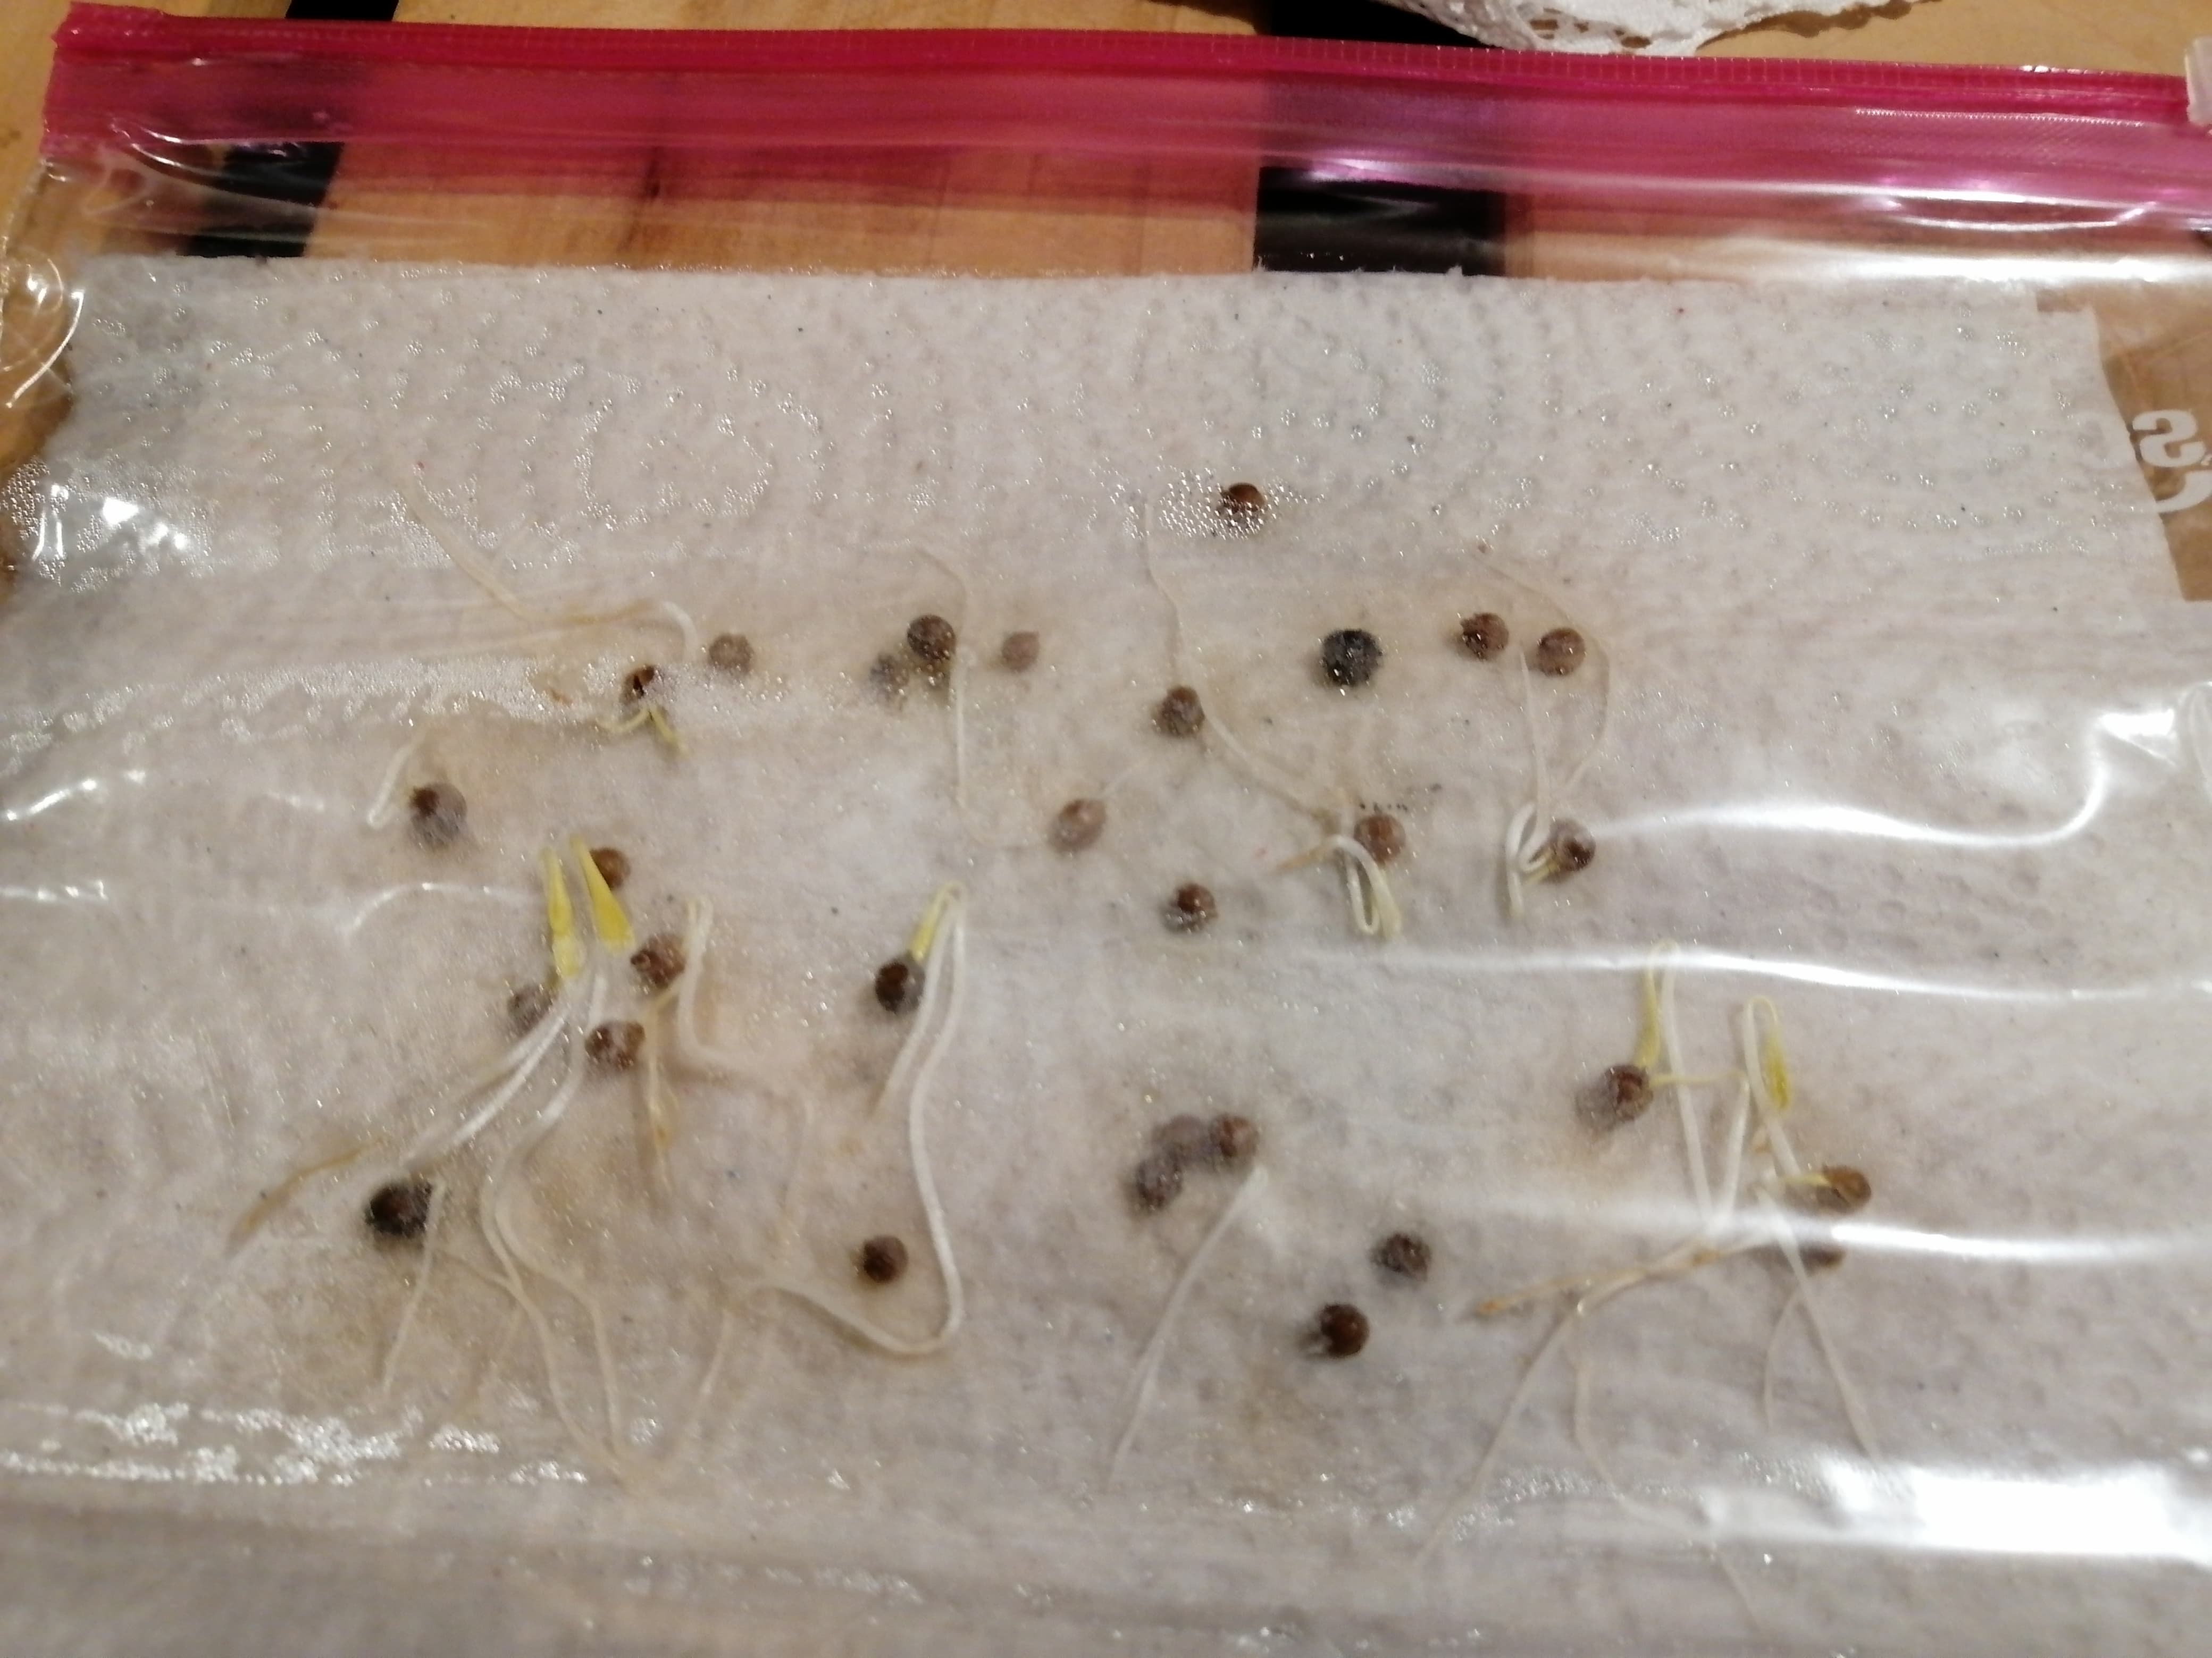
\includegraphics[scale= 0.05]{Germinacion_ziplock.jpg}
	\caption{Semillas germinadas utilizando papel toalla y bolsa resellable.}
	\label{fig:ziplock}
\end{figure}

\begin{figure}[H]
	\centering
	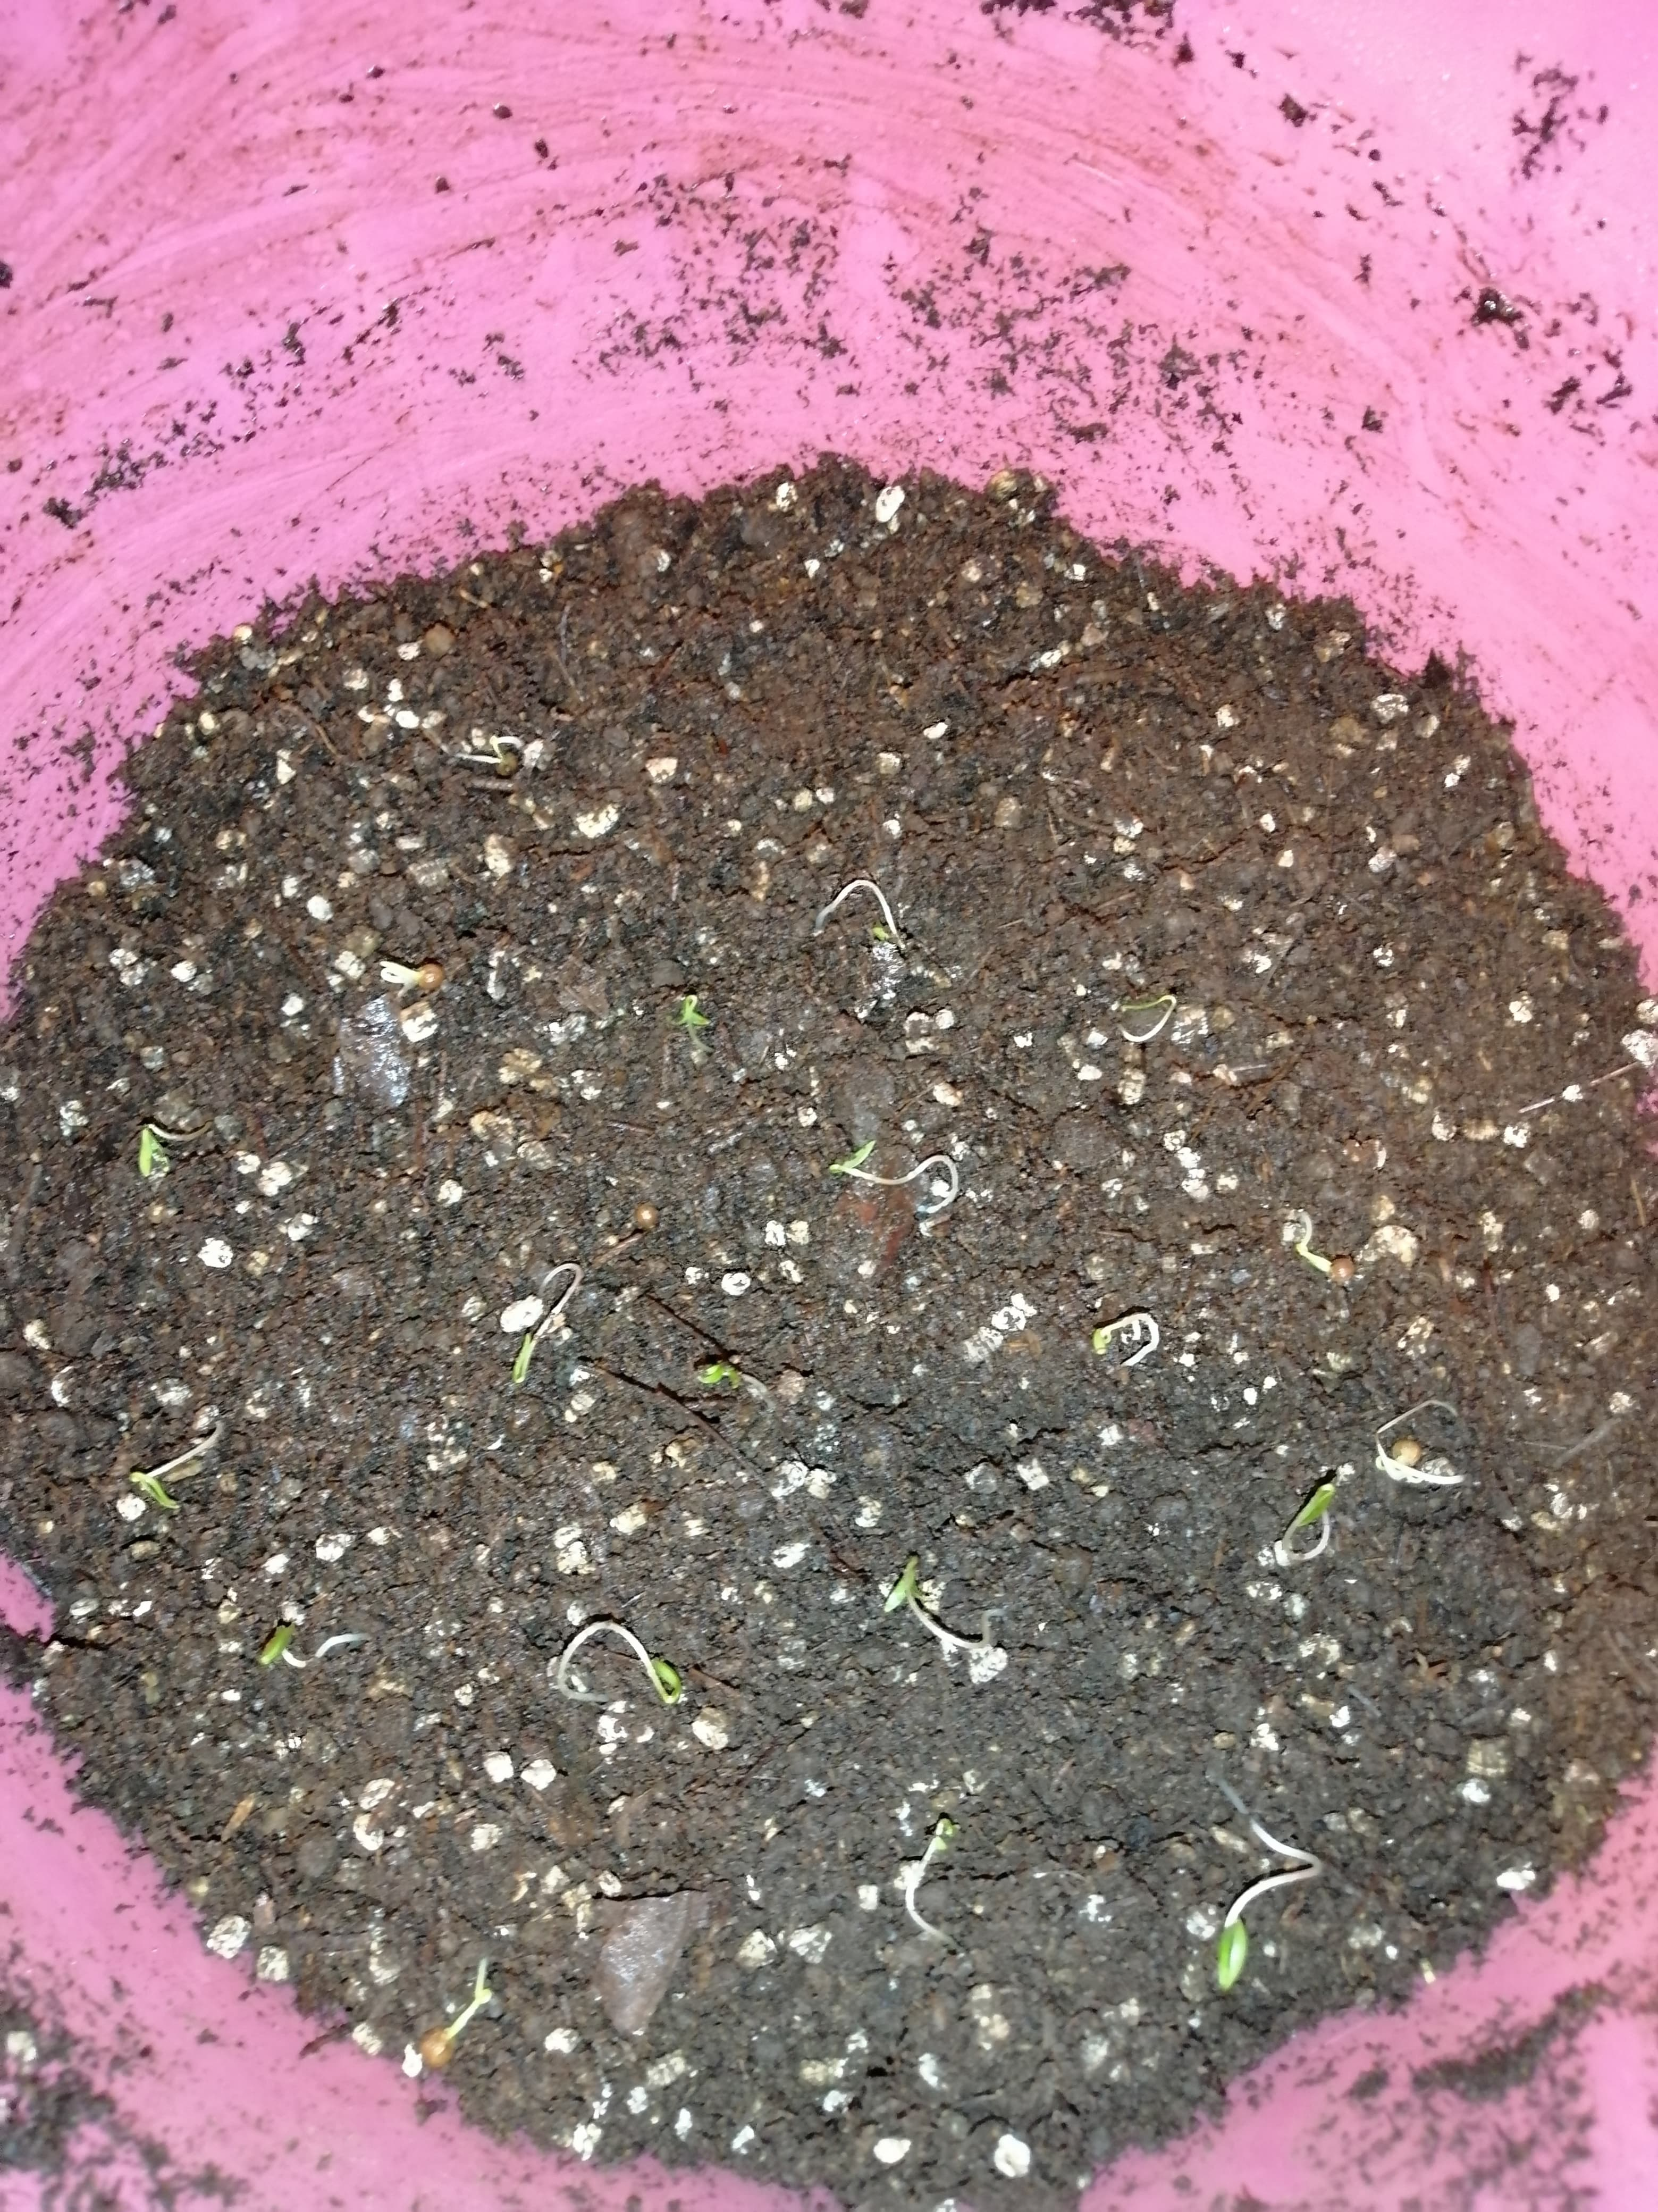
\includegraphics[scale= 0.05]{Germinacion_peatmoss.jpg}
	\caption{Semillas germinadas utilizando sustrato mecánico inerte.}
	\label{fig:peatmoss}
\end{figure}

Tanto las semillas en la bolsa resellable como las del sustrato inerte presentaron desarrollo de raíces luego de 8 días en condiciones óptimas. Es importante mencionar que si bien el sustrato inerte fue capaz de mantener un nivel de humedad aceptable, fue necesario regar dicho sistema de manera periódica durante el tiempo de germinación. Por otro lado, las semillas dentro de la bolsa resellable nunca presentaron pérdidas significativas de humedad, por lo que no fue necesario hidratarlas más de una vez. A parte de la diferencia en retención de humedad, no se observó una diferencia significativa entre ambos métodos de germinación en cuanto al tiempo o eficiencia. 

\subsection{Retos en el desarrollo de retoños}

Una vez se observó el desarrollo de raíces en los retoños, estos se trasladaron a un sustrato compuesto principalmente por \textit{peat-moss}, vermiculita y tierra abonada. Es importante resaltar que durante las primeras semanas de desarrollo, los retoños no recibieron una cantidad adecuada de luz, por lo que se presentó un fenómeno conocido como \textit{bolting} o espigado. Este proceso llevó al desarrollo de tallos largos y débiles, lo cual llegó a representar un reto significativo en futuras etapas del desarrollo. Adicionalmente, durante las primeras semanas de crecimiento, se utilizó una proporción menor de compost, lo cual redujo la cantidad de nutrientes disponibles para los retoños.

\subsection{Transplante de retoños a sustrato nutritivo de crecimiento}

Los retos mencionados anteriormente se corrigieron luego de transplantar los retoños al sustrato nutritivo, sin embargo, la mayoría de los retoños contaban con un tallo principal considerablemente largo y débil. Por esta razón, se sembraron los retoños a una mayor profundidad, buscando evitar la pérdida de retoños por daños al tallo. Mientras que este proceso ayudó a que la mayoría de los retoños se continuaran desarrollando, la exposición a los elementos como la lluvia y el viento inevitablemente dobló algunos de los retoños, llevando a pérdidas por falta de circulación de nutrientes a través de los tallos. En la Figura \ref{fig:transplante_plantas}, se observa la configuración de los retoños en las macetas, y se acortó la altura de los tallos al sembrarlos a mayor profundidad. Finalmente, es importante mencionar que durante el proceso de transplante, se descartaron aquellos retoños que se habían vencido sobre su propio peso, así como retoños que no habían desarrollado suficientemente sus raíces como para absorber nutrientes del sustrato.

\begin{figure}[H]
	\centering
	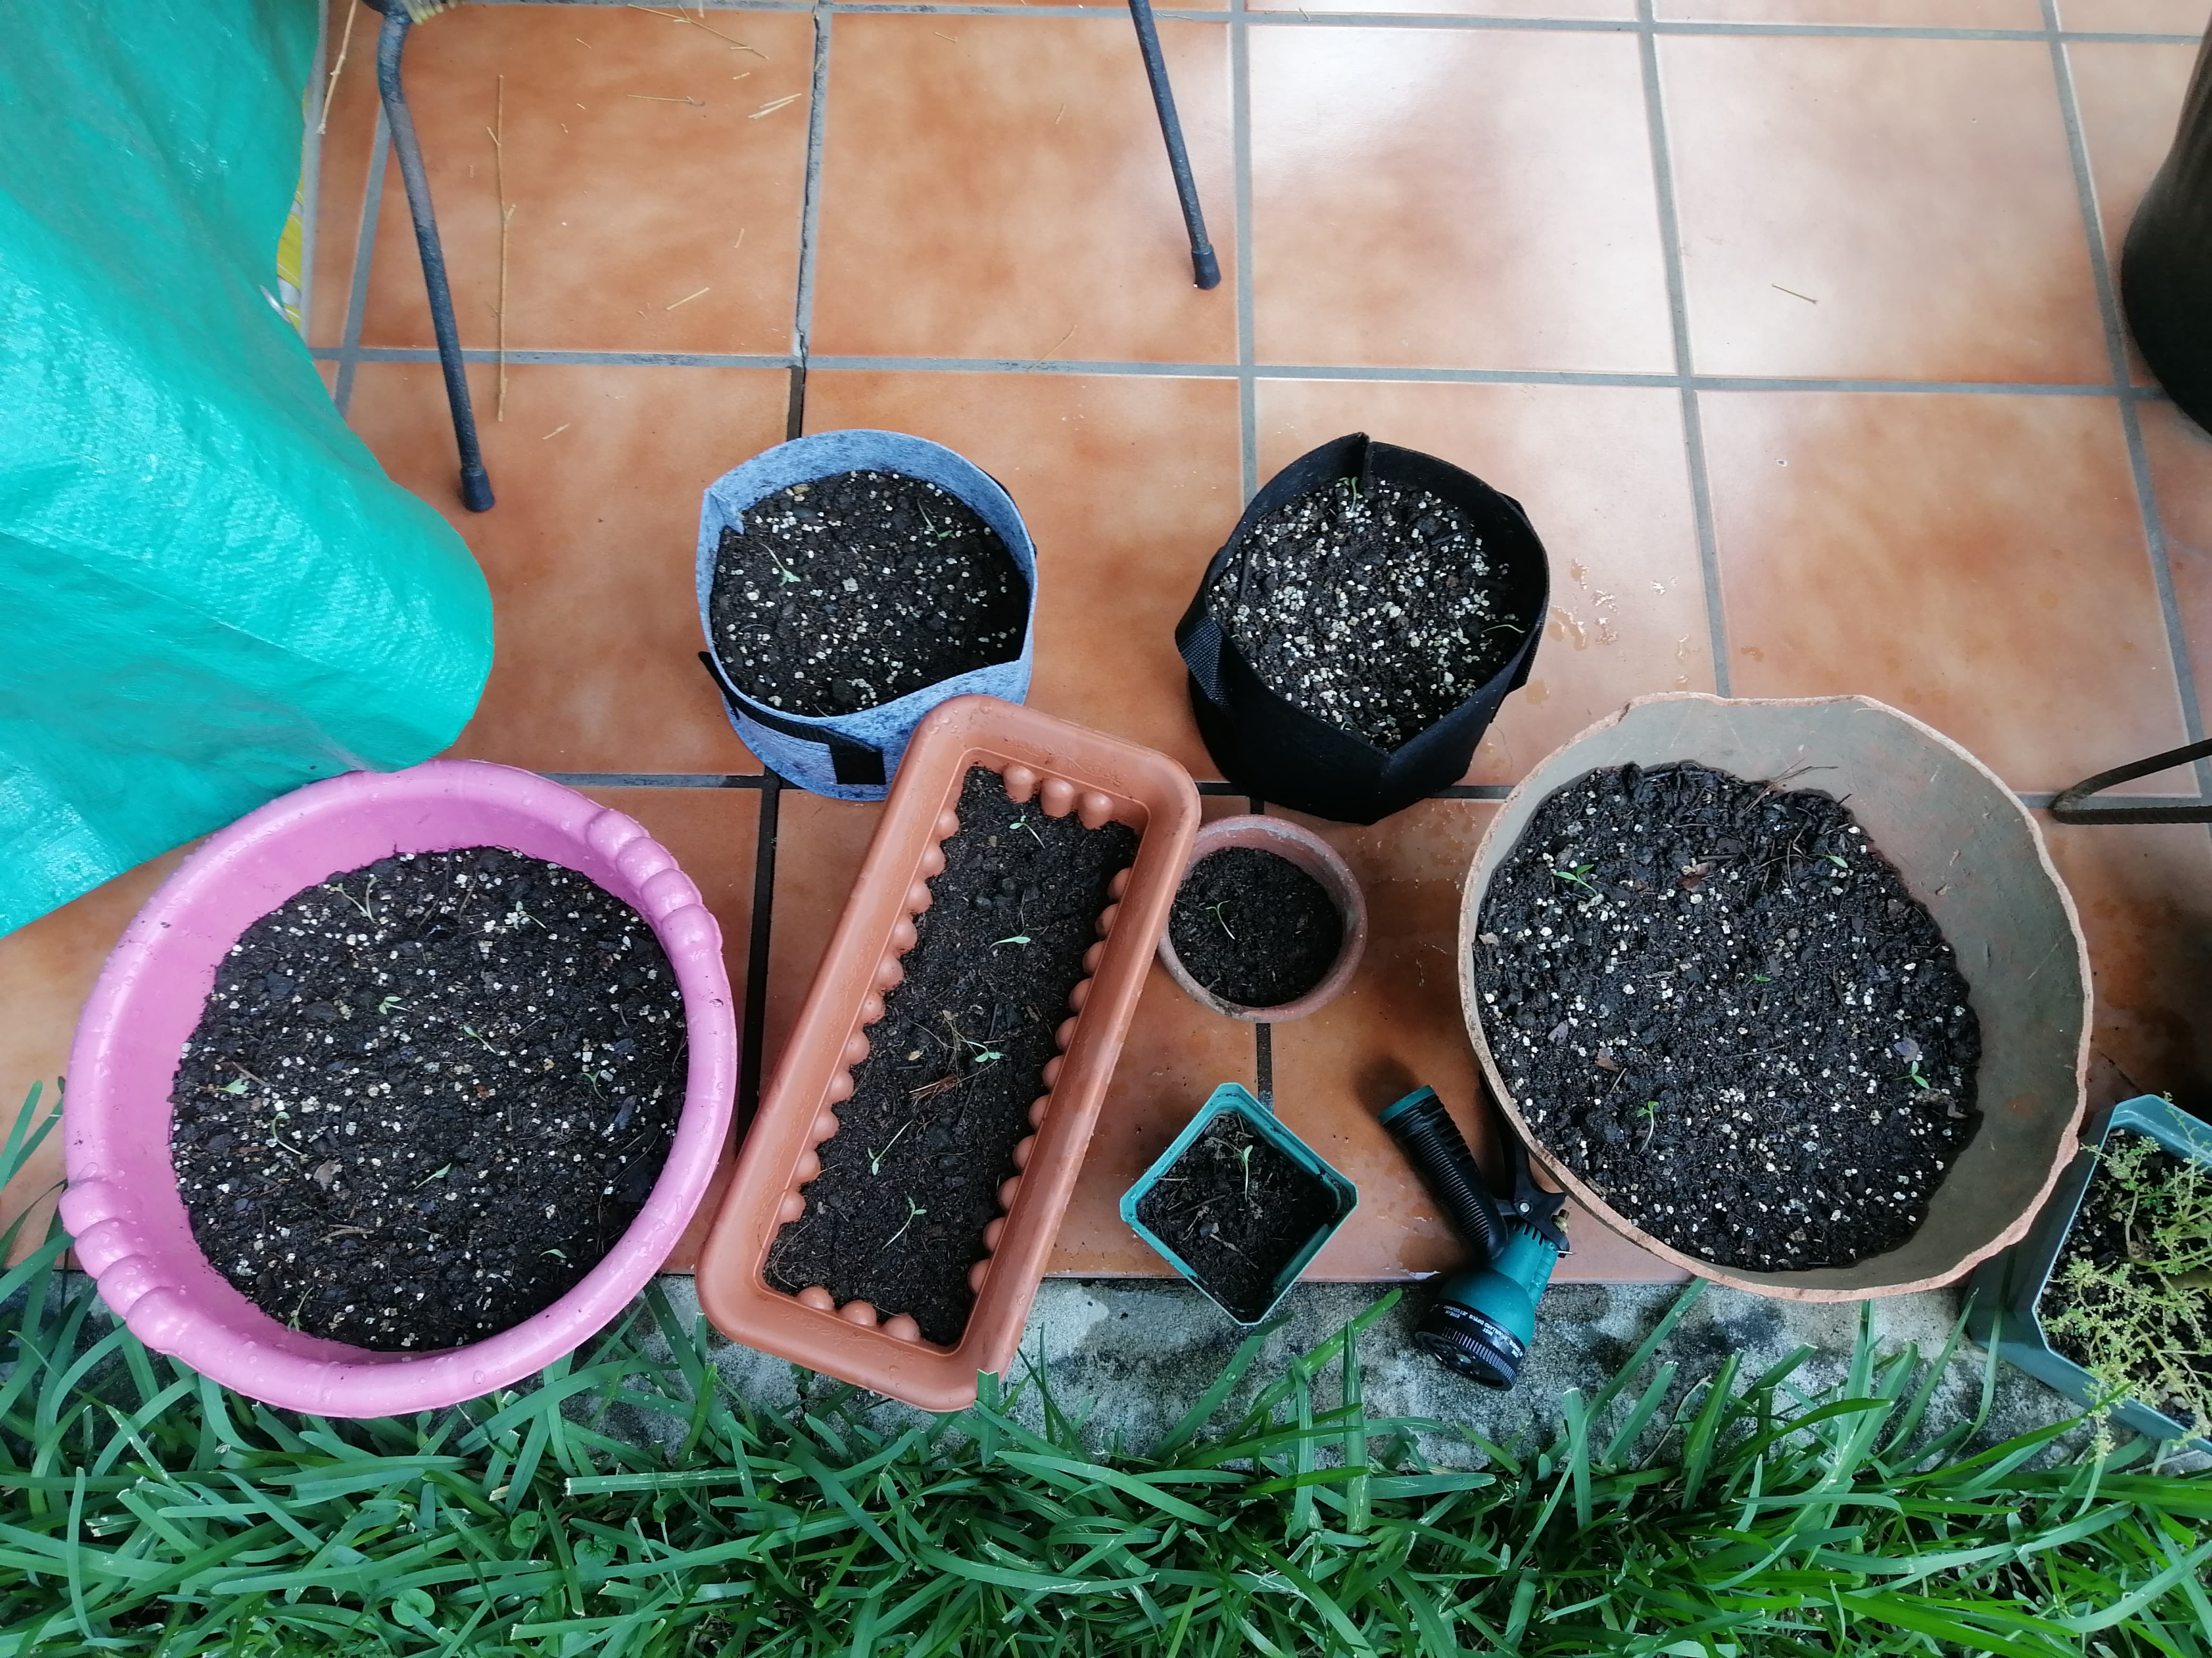
\includegraphics[scale= 0.05]{Retonos_transplantados.jpg}
	\caption{Configuración de los retoños luego de ser transplantados a sustrato nutritivo de crecimiento.}
	\label{fig:transplante_plantas}
\end{figure}


\section{Cultivo de cilantro en sistema hidropónico}

Luego de las primeras 4 semanas del desarrollo del cilantro en sustrato de crecimiento, se trasladaron 12 plantas de cilantro al sistema hidropónico. Se colocó una planta por espacio disponible en los canales de crecimiento, y se reguló la concentración de solución nutritiva, diluyendo 2.5 mL de macro y micro nutrientes por galón de agua en el sistema. Ahora bien, cabe mencionar que en el momento en que se trasladaron las plantas de cilantro, aún no se contaba con un control adecuado de temperatura ambiente. Adicionalmente, como se observa en la Figura \ref{fig:estructura_final}, el sistema tampoco contaba con un control de luz de crecimiento, estando abierto aún a la luz ambiental.

\subsection{Elementos de soporte para las plantas}

En un sustrato activo, este provee tanto los nutrientes necesarios para el crecimiento de las plantas, como la estabilidad mecánica para asegurar que estas se mantengan erguidas. Ahora bien, en un sistema hidropónico, las plantas no cuentan con este sustrato, por lo cual es necesario utilizar otros métodos para brindar estabilidad mecánica a las plantas. Durante las pruebas iniciales, se utilizaron pedazos de tubo flotador, los cuales se cortaron de manera que fuesen capaces de ingresar en los agujeros disponibles en los canales de crecimiento. Además, se aseguró que estos fueran capaces de apoyar a las plantas, asegurando que se mantuvieran en su lugar. Ahora bien, cabe mencionar que estos tubos flotadores están elaborados de un material sintético el cual absorbe e irradia calor con facilidad. Esto no habría sido un gran problema en un sistema hidropónico sumergible, sin embargo, al utilizar la metodología NFT, este material no contó con una manera de liberar su calor.

Mientras se realizaron pruebas iniciales de crecimiento, se observó una temperatura máxima en el sistema alrededor de los 32 °C, la cual fue considerablemente mayor a la temperatura máxima del cilantro, alrededor de los 25 °C. Este aumento en temperatura elevó el consumo de agua de las plantas, resultando en una acumulación de sales en las raíces, como se observa en la Figura \ref{fig:raices}. Esta acumulación de sales, junto a las elevadas temperaturas en los pedazos de tubo flotante, llevaron a la pérdida del 66\% de las plantas en el sistema hidropónico.

\begin{figure}[H]
	\centering
	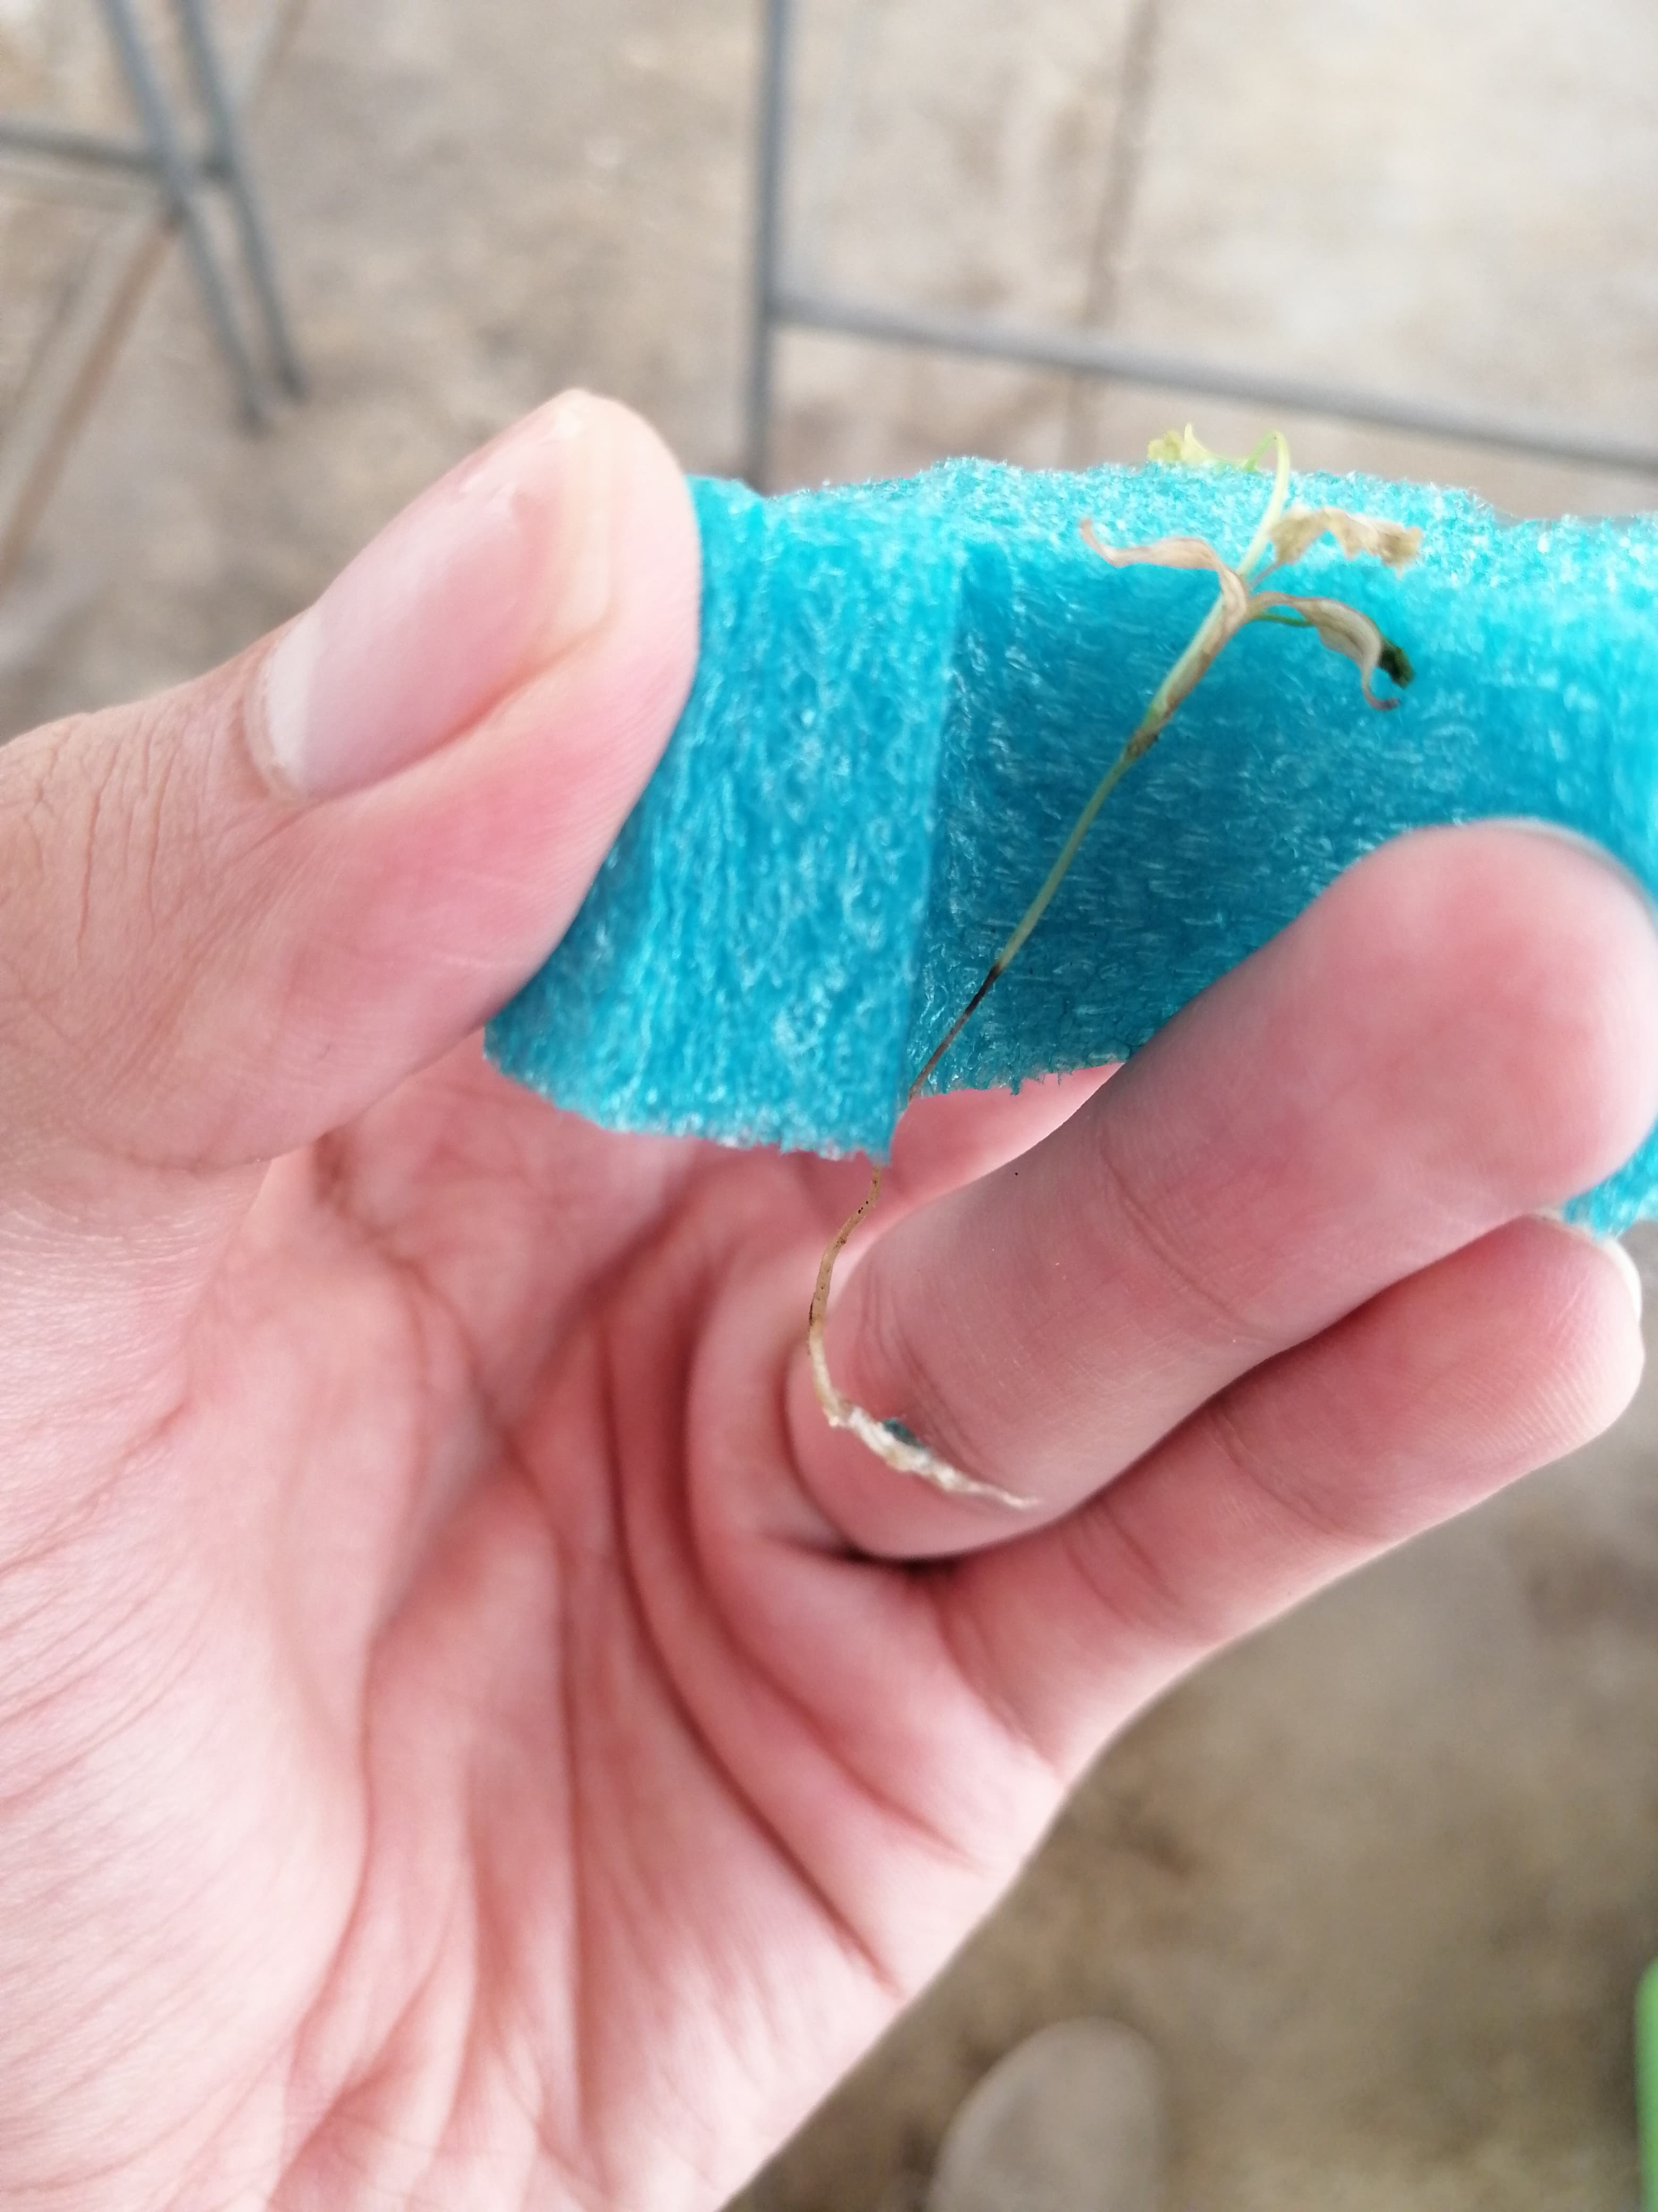
\includegraphics[scale= 0.05]{Sales_raices.jpg}
	\caption{Retoño de cilantro con tallo seco y raíces bloqueadas por sales de la solución nutritiva.}
	\label{fig:raices}
\end{figure}

\section{Retos en el cultivo del cilantro durante períodos de prueba}	% [==========MISSING==========]

\section{Comparaciones del crecimiento del cilantro}	% [==========MISSING==========]

